\documentclass[10pt, a4paper]{memoir}

%--------------------------------------------------------- Style setup ---------------------------------------------------------
\aliaspagestyle{cleared}{plain}

%--------------------------------------------------------- Package Setup ---------------------------------------------------------

\usepackage[utf8]{inputenc}
%\usepackage{textcomp} %Use for old MiKTex framework with updates packages
%\usepackage{lmodern} %Modern font
%\usepackage[T1]{fontenc} %T1 Font
\usepackage{amsmath, amsthm, amssymb} %Gives math tools and environments
\usepackage{mathtools} %Extensions to amsmath
\usepackage{mathrsfs} %Provide \mathscr command
\usepackage{nccmath} %Improve space of \displaybreak and more
\usepackage{graphicx} %Include graphics
\usepackage{datetime} %Datetime
\usepackage{advdate} %\today
\usepackage{verbatim} 
\usepackage[english]{babel}
\usepackage{gensymb} %\degree, \celsius, etc.
\usepackage{bm} %\bm
\usepackage{float} %Add H float modifier
\usepackage{wasysym } %Contradiction arrow
\usepackage{enumitem} %Add control to enumerate environment
\usepackage{xpatch}  %\better declaration
\usepackage{capt-of} %\captionof for something not a float
\usepackage{caption}
\usepackage{pdfpages} %Add multipage pdf document option
\usepackage{color}
\usepackage{geometry}
\usepackage[noanswer]{exercise} %Add exercise environment

\usepackage{esdiff} %Add easy diff by \diff
\usepackage{fancyhdr} %Used for building footers and headers
\usepackage{courier} %Courier font
%\usepackage{framed} %Create framed, shaded and leftbar environment
\usepackage{mdframed} %Same as framed just add breakable framed and coloured boxes
%\usepackage{lipsum} % for creating dummy text
\usepackage{cancel} %Used for \cancel that draws a slash through its argument.
\usepackage{collectbox} %\savebox
\usepackage[most]{tcolorbox} %Add coloured boxes
\usepackage{varwidth} %varwidth enviorment is minipage where width is a maximum value
\usepackage{physics}
\usepackage{nameref}%\nameref
\usepackage{siunitx}
\sisetup{exponent-product = \cdot,per-mode=reciprocal-positive-first}
\usepackage{braket} %Add braket notation
\addto\captionsdanish{%
}
\usepackage{hyperref} %Load last ALWAYS
\usepackage{titlesec} %Change space of sections and subsections
\usepackage{cleveref}
\usepackage{pgfplots}

\usepackage{listings}


%--------------------------------------------------------- Theorems setup ---------------------------------------------------------
\numberwithin{equation}{section}
\newtheoremstyle{defp}% name
{}% Space above
{}% Space below
{}% Body font
{}% Indent amount1
{\bfseries}% Theorem head font
{\newline}% hPunctuation after theorem head
{0.1em}% Space after theorem head2
{}% Theorem head spec (can be left empty, meaning `normal')

\newtheoremstyle{defq}% name
{1em}% Space above
{}% Space below
{\itshape}% Body font
{}% Indent amount1
{\bfseries}% Theorem head font
{\newline}% hPunctuation after theorem head
{}% Space after theorem head2
{}% Theorem head spec (can be left empty, meaning `normal')

\newtheoremstyle{dotless}%
{}%
{}%
{\itshape}%
{}%
{\bfseries}%
{\newline}%
{1em}%
{}%

\makeatletter
\renewenvironment{proof}[1][\proofname]{\par
    \normalfont \topsep6\p@\@plus6\p@\relax
    \trivlist
    \item[\hskip\labelsep
        \itshape
        #1\@addpunct{.} \newline] }%\ignorespaces}
\makeatother

\renewcommand*{\proofname}{Proof}

\theoremstyle{plain}
\newtheorem{thm}{Theorem}

\theoremstyle{defp}
\newtheorem{de}[thm]{Definition}

\theoremstyle{dotless}
\theoremstyle{definition}
\newtheorem*{eks}{Example}
\theoremstyle{dotless}
\newtheorem{st}[thm]{Theorem}
\theoremstyle{dotless}
\newtheorem{lem}[thm]{Lemma}
\theoremstyle{defp}
\newtheorem{po}{Postulat}
\theoremstyle{defp}
\newtheorem*{ko}{Konstuktion}
\makeatletter
\patchcmd{\th@be}{\thm@headfont{\itshape}}{\thm@headfont{\normalfont}}{}{}
\makeatother
\theoremstyle{be}          % in order to avoid content to be printed in italics
\newtheorem*{be}{Note} 
\theoremstyle{defp}
\newtheorem*{no}{Notation}
\makeatletter
\renewenvironment{proof}[1][\proofname]{\par
  \pushQED{\qed}%
  \normalfont \topsep6\p@\@plus6\p@\relax
  \trivlist
  \item[\hskip\labelsep
        \itshape
%    #1\@addpunct{.}]\ignorespaces% DELETED
    #1]\ignorespaces% ADDED
}{%
  \popQED\endtrivlist\@endpefalse
}
\makeatother

%\usepackage{ucs,babel} %No idea
%\usepackage[all,cmtip]{xy} %No idea


%--------------------------------------------------------- Own Definitions ---------------------------------------------------------
\makeatother %Create double underline
\def\doubleunderline#1{\underline{\underline{#1}}}

\makeatletter %Better arrays
\renewcommand*\env@matrix[1][*\c@MaxMatrixCols c]{%
  \hskip -\arraycolsep
  \let\@ifnextchar\new@ifnextchar
  \array{#1}}
\makeatother

%Create equality symbol with some text variable that get set above the equation
\newcommand\myeq{\mathrel{\overset{\makebox[0pt]{\mbox{\normalfont\tiny\sffamily def}}}{=}}}

\newcommand{\BAR}{% Own bar definition
  \hspace{-\arraycolsep}%
  \strut\vrule % the `\vrule` is as high and deep as a strut
  \hspace{-\arraycolsep}%
}

\newcommand{\ch}{\cosh}
\newcommand{\sh}{\sinh}
\newcommand{\tnh}{\tanh}
\newcommand{\Arcosh}{\operatorname{Arcosh}}
\newcommand{\Arsinh}{\operatorname{Arsinh}}
\newcommand{\Artanh}{\operatorname{Artanh}}
\newcommand{\ord}{\operatorname{ord}}
\newcommand\nm[1]{\left\lVert#1\right\rVert}
\DeclarePairedDelimiter\abss{\lvert}{\rvert}
\renewcommand{\epsilon}{\varepsilon}
\renewcommand{\phi}{\varphi}
\newcommand\lf[1]{\left(#1\right)}
\newcommand\pr[1]{#1^\prime}
\newcommand\lfa[1]{\langle#1\rangle}
\newcommand\lff[1]{\left[#1\right]}
\newcommand\mb[1]{\mathbb{#1}}
\newcommand\mc[1]{\mathcal{#1}}
\newcommand\code[1]{\texttt{#1}}
\newcommand\inproc[1]{\langle#1\rangle}
\DeclarePairedDelimiter\ceil{\lceil}{\rceil}
\DeclarePairedDelimiter\floor{\lfloor}{\rfloor}
\newcommand\ttt[1]{\texttt{#1}}
\newcommand\tsc[1]{\textsc{#1}}
\newcommand{\CS}{C\nolinebreak\hspace{-.05em}\raisebox{.6ex}{\tiny \#}}

\newcommand\type[1]{\ttt{\textcolor{green}{#1}}}

%--------------------------------------------------------- Computer Science Setup ---------------------------------------------------------

\usepackage{forest}
\usepackage{adjustbox}
\usepackage{algorithm}
\usepackage[noend]{algpseudocode}

\algrenewcommand{\algorithmicrequire}{\textbf{Input:}}
\algrenewcommand{\algorithmicensure}{\textbf{Output:}}
\algnewcommand\An{\textbf{ And } }
\algnewcommand\Or{\textbf{ Or } }
\algnewcommand\To{\textbf{ to } }

\let\oldReturn\Return
\renewcommand{\Return}{\State\oldReturn}

%for at lave  i align enviorment
\makeatletter
\let\save@measuring@true\measuring@true
\def\measuring@true{%
  \save@measuring@true
  \def\beamer@sortzero##1{\beamer@ifnextcharospec{\beamer@sortzeroread{##1}}{}}%
  \def\beamer@sortzeroread##1<##2>{}%
  \def\beamer@finalnospec{}%
}
\makeatother

%pause efter hvert ligning
\makeatletter
\g@addto@macro\normalsize{%
    \setlength\belowdisplayskip{2pt}
}

\makeatletter
\g@addto@macro\normalsize{%
    \setlength\abovedisplayskip{7pt}
}

%Lille o notation \smallO
\newcommand\smallO{
  \mathchoice
    {{\scriptstyle\mathcal{O}}}% \displaystyle
    {{\scriptstyle\mathcal{O}}}% \textstyle
    {{\scriptscriptstyle\mathcal{O}}}% \scriptstyle
    {\scalebox{.7}{$\scriptscriptstyle\mathcal{O}$}}%\scriptscriptstyle
  }

\usepackage{chngcntr}
\counterwithout{equation}{section} % remove the chapter number
% \counterwithin{equation}{section}  % add the chapter number

\usepackage[newfloat]{minted}

\definecolor{mauve}{HTML}{E0B0FF}

\definecolor{codegray}{gray}{0.85}
\newcommand{\codes}[1]{\colorbox{codegray}{\texttt{#1}}}


\usepackage{chngcntr}
\counterwithin{Exercise}{section}



%--------------------------------------------------------- Tikz setup ---------------------------------------------------------
%#\usetikzlibrary{positioning}

%--------------------------------------------------------- lst setup ---------------------------------------------------------

\definecolor{key}{HTML}{00FF00}
\definecolor{val}{HTML}{0000BB}

\lstdefinelanguage{WowAPI}{
	keywords={Type, Null},
	keywordstyle=\color{key}\bfseries,
	keywords=[2]{String, Int, Char, Boolean},
	keywordstyle=[2]\color{val}\bfseries,
	sensitive=true,
	morecomment=[l]{//}
}

\lstset{language=WowAPI,
	basicstyle=\footnotesize, 
	numbers=left,
	numberstyle=\tiny\color{gray},
	stepnumber=1,    
	firstnumber=1,
	numbersep=5pt,
	numberfirstline=true,
	frame = single,
	breaklines=true,
	tabsize=4,
	commentstyle=\color{gray},
	stringstyle=\color{orange}
}

%--------------------------------------------------------- Beginning of document ---------------------------------------------------------
\setlength\parindent{0pt}

\renewcommand{\ExerciseHeader}{\large\textbf{\ExerciseName~\ExerciseHeaderNB} \smallskip\newline}
\renewcommand{\AtBeginExercise}{\hspace{-0.66em}}
\renewcommand{\AnswerHeader}{\large\textbf{\AnswerName~\ExerciseHeaderNB}\smallskip\newline}
\setlength\AnswerSkipBefore{1em}


\setlength\arraycolsep{2 pt}
\setcounter{tocdepth}{2}
\setcounter{secnumdepth}{3}

\titlespacing*{\section}
{0pt}{3ex plus 1ex minus .2ex}{1ex plus .5ex}

\titlespacing*{\subsection}
{0pt}{1ex plus 0.5ex minus .2ex}{1ex plus .2ex}

\openany


\hypersetup{%
    pdfborder = {0 0 0}
}

\usepackage{csquotes}

\usepackage[authordate,backend=bibtex, bibencoding=utf8]{biblatex-chicago}
\addbibresource{ref.bib}

%Styling of quotes
\usepackage{etoolbox}
\AtBeginEnvironment{quote}{\par\singlespacing\small}

\begin{document}

%--------------------------------------------------------- Document Setup ---------------------------------------------------------

\newcommand*\mytitle{\textsc{Software Requirements for ReunionLog}}


\title{\mytitle \\[1ex] \large \textsc{Reunion}\\}
%\date{\AdvanceDate[0]\today \\ }
\date{}

\centering
\maketitle
	{\scshape\LARGE \LaTeX \par}
	\vspace{0.5cm}
	{Lead Programmer and Lead Designer - \Large\scshape Nickgismokato\par}
	\vspace{0.3cm}
	{Design contributor - \Large\scshape Bj\par}
	\vspace{0.3cm}
	{Design contributor \& tester - \Large\scshape Casper\par}
	\vspace{1cm}
	\vfill
	Written by\par
	~Nick \textsc{Laursen}


\thispagestyle{empty}

\newpage

\section*{\centering Preface}

%\raggedright
This is the documentation of the requirements we want to follow when creating the program \textsc{ReunionLog}. We will be following the \textsc{SOLID} principles. This software is a program meant for the guild \textsc{Reunion} in the game \textsc{World Of Warcraft}. This software will use the \ttt{API} from \textsc{WarcraftLogs}. 

\medskip

Most of these requirements have been gathered from multiple months of pre-gathering data from the \textsc{WarcraftLogs} \ttt{API}. This has been done by creating a \textit{proof-of-concept} program with \textsc{Python}.

\medskip

\center

This software is under the \textsc{MIT License}. Read \ttt{LICENSE} for more information.


\tableofcontents

\newpage

\raggedright

\pagestyle{fancy}
\renewcommand{\sectionmark}[1]{\markboth{#1}{}}

\fancyhf{}
\rhead{\fancyplain{}{$ $\leftmark $ $}} % predefined ()
\lhead{\fancyplain{}{$ $\mytitle$ $}} % 1. sectionname, 1.1 subsection name etc
\cfoot{\fancyplain{}{\thepage}}
\fancypagestyle{plain}{%
  \fancyhf{}%
  \fancyfoot[CF]{\thepage}
  \renewcommand{\headrulewidth}{0pt}%
}

%--------------------------------------------------------- Document ---------------------------------------------------------

\chapter{\textsc{WarcraftLogs} and the \ttt{API}}

\section*{Abstract}

This chapter will go through \textsc{WarcraftLogs} and the \ttt{API} correlating. For this chapter we will not go through the actual documentation but rather give a short refer to the documentation and lay out the most important aspect from the site and the \ttt{API}

\section{Website}

The website for \textsc{WarcraftLogs}\footnote{\url{https://www.warcraftlogs.com/}} is a popular website used by guilds to gather data to one single site. This is done though multiple addons and their own in-house software. 

\subsection{Overall form}

The data than can be collected is both in the form of \textsc{Guild} data, \textsc{Raid} data, \textsc{Dungeon} data, \textsc{Character} data and much more. These can be accessed for all through the website. This can be done by everyone anonymously.

\medskip

The website uses \textsc{graphQL} to display most of their data. Both in tables both also in graphs and tables containing graphics. This gives an easier overview for most users. They to also have some options you can choose for the specific data you want to be showed. 

\medskip

A downside to this approach is that a lot of the specific options is not showed. One could reason the "\textit{simpler}" design is because they want all users to use their website, no matter their technical background. 

\subsection{Specific to our needs}

What described in \textbf{Section 1.1.1} sound really great and reasonable useful for most users case. This is indeed the case for most users, but if you want the information not available on the site or you want another way to represent the data, then the site is not for you. This is why we will be using the data given to us by the \ttt{API}.

\medskip

The only need we have of the website is to check if the information we get is also the information displayed on the site.  

\section{Documentation for the \ttt{API}}\label{sec:Doc}

The \ttt{API} and it's documentation is, for a lack of a better word, idiotic made. There exists two \ttt{API}'s. Version 1 and version 2. We will be using the latter. This version has "\textit{better}" documentation than it's counterpart and uses \textsc{OAuth 2.0} for it's \ttt{API} authentication. The documentation can be found two places. For authentication documentation you can find it at \cite{AuthLink} and you can find the actual command call documentation at \cite{DocLink}.

\subsection{\textsc{GraphQL}}

The first thing we should worry about is the authentication. As mentioned in the \textbf{Preface} we have already made successful connection, therefore this will be discussed later.  

\medskip

\textsc{GraphQL} is the schema of how to make calls to the \ttt{API}. This is done by sending you authentication and a "\textit{Query}" call. This is in simple terms just a string with specific data. This data is both used to tell \textsc{WarcraftLogs} server what you would like to receive bout also where in the schema the server would have to lookup this data. Clearly there is a need to create these query strings. 

\medskip

Therefore we will be using \ttt{GraphQL} library from \textsc{Graphql-dotnet}. More information can be found at \cite{GQLdotnet}. If you were to look at \cite{DocLink} you would find there is a lot of commands you can send. Therefore it is important to create an object which can be agile and create all the necessary strings which we will be using.  

\subsection{Limitation of the \ttt{API}}

When it comes to the \ttt{API} a lot of limits start to show. Some in the documentation and some in the actual \ttt{API} itself. Let us start talking about the \ttt{API} itself. When on a free tier, i.e not subscribed to \textsc{WarcraftLogs} website, you can at maximum make 3.600 calls to their server pr. hour. This inherently doesn't sound that bad, but you will later see in depths why this is a bad system. 

\medskip

I will agree that this stops most novice \ttt{DDOS} attacks to their server, but since the introduction of the second version of their \ttt{API}, multiple clients can easily be set up and could potentially help in the \ttt{DDOS} attacks. Let us now explain why this rate limit is bad when you want to make a software that pulls a great amount of data. 

\medskip

Let us say you had a guild that was raiding and you both raided \textsc{Mythic} and \textsc{Heroic} during the same log. Let us furthermore assume you want the data for when they die and how many pulls they were on, but only for the mythic. By scouring through their schema documentation (\cite{DocLink}), you find the \ttt{Report} object inside the documentation. This is essentially what you want. So you create a query string with \ttt{report} as first argument and and then you scour through the documentation and find the \ttt{event} option which deliver a \ttt{ReportEventPaginator} which is just a list event in the log file. This gets returned as data in form of a \ttt{JSON} string. Let us see the documentation for it:

\begin{displayquote}[\cite{DocLink}]
"A set of paginated report events, filterable via arguments like type, source,t arget, ability, etc. This data is not considered frozen, and it can change without notice. Use at your own risk."
\end{displayquote}

This object has an argument you can filter from called \ttt{difficulty}. The documentation for this is as follow:

\begin{displayquote}[\cite{DocLink}]
"\textbf{difficulty}: Optional. Whether or not to filter the fights to a specific difficulty. By default all fights are included."
\end{displayquote}

This is brilliant. We can now filter our \ttt{Event} to mythic only. Later down the line is argue that \ttt{difficulty} is an integer value. Great so now we just need to figure our what integer value. This is the first hurdle we found when trying this. No actual documentation is given for the arguments, except if it is an object or enum type which they have created. So we set up in \textsc{Python} a script to run through with value $n$ where $n\in\set{-1000,-999,\dots,999,1000}$. Then we checked if there where any difference between the \ttt{JSON} strings we received and we got that there was no difference for any $n$ value. 

\medskip

Clearly any user would be confused. Why would an \ttt{API} give you an option and then not document said option and actually do nothing with this option. Your first instinct would now be to contact  \textsc{WarcraftLogs}. So you write them an email and there response they send you back can be seen in \cref{fig:MailSupp}. So you go to their discord find the thread about the \ttt{API} and ask you question. The intention of this documentation is not to out anyone from their support team and therefore I will not share the conversion I had. But trust us when we say that if was probably the most useless information and support we have ever received. 

\medskip

So how did we fix it, you may ask? We looked at the documentation and again read what was written under the \ttt{difficulty} argument. The difficulty argument says it filter fights. So we then took a look at the \ttt{ReportFight} object. We tested this and sure enough it worked. So to simplify what we now have to do if we wish to get the event data only for \textsc{Mythic}. First we need to get all the fight data that had that difficulty i.e the \ttt{fightIDs}. This is done with the \ttt{ReportFlight} object. Then we have to sort our \ttt{ReportEventPaginator} to the \ttt{fightIDs}. Now we have used two calls of our 3.600 rate limit.

\medskip

In our demo in \textsc{Python} it became clear that we also had to pull a lot more data than just fight i.e pulls and so on. We now have to pull every single fiights, every single name from that fight and the event itself. This gives us a rough estimate:

$$l\cdot\lf{a_{\text{Fights}}+a_{\text{Event}}+a_{\text{name}}\cdot p},$$
where $p$ is the amount of players in any fights and $l$ is the amount of different logs we want to pull data from. Since we cannot get \ttt{fightIDs} whilst also getting the event to only get data from the mythics, we would need to do this over two separate calls and also we cannot pull names just from the event log the way we want it, so we have to do it separately. 

\medskip

This is probably the most irritating limit of the \ttt{API} and therefore we would need to make sure our software can handle this limit in case our request limit get met.


\section{Integration from the \ttt{API} to C\ttt{\#}}

As discussed in \ref{sec:Doc} it is clear that we would need many objects to handle everything involving \tsc{WarcraftLogs} \ttt{API} and it's authentication. Clearly we would need objects handling our query strings, \textit{all of them}, handling of the authentication and most importantly handling the data we receive after we have made a call, i.e the response.

\subsection{Authentication}

Creating an authentication for our software is actually quite easy. We don't need any libraries for the creation of the code or the requester. The only thing we need is an users \ttt{client\_id} and \ttt{client\_secret}. The \ttt{tokenURL} is a constant i.e "\textit{https://www.warcraftlogs.com/oauth/token}". Everything else is user input. This is also important but will be dealt with differently.

\medskip

We will need the user to create the \ttt{client\_id} and \ttt{client\_secret} which we will save as local data for further use. This will be done at first time use of the software.

\subsection{Query Strings}

When dealing with query strings within this \ttt{API}, you are in fact dealing with a \ttt{json} call within the \tsc{GraphQL} schema. As noted in \textbf{Section 1.2.1 GraphQL}, we will be using the \ttt{GraphQL} library from \ttt{Graphql-dotnet} (\cite{GQLdotnet}). This library is also under the \tsc{MIT} license, so no issue in license agreements here. It is important to note that \tsc{Facebook} created \tsc{GraphQL}. This library is just an implementation to \tsc{.NET}. You can easily install it by the following command:

\begin{minted}{bash}
$ dotnet add package GraphQL
\end{minted}

This is the only package needed for this library. We don't need serialization or document cashing since we will implement it ourself if needed. 

\subsection{Data extracted from the \ttt{API}}

After we have made a call, you would think we are done. Clearly this isn't the case. The \ttt{JSON} is what our call return. This data is not just a "pure" \ttt{JSON} string. It has layers within its own index. Therefore we need to go through these index layers if we wish to get to the actual data we need. This could either be implemented in the call function or in it's own class.

\medskip

We will implement this within its own class. The main reason is we don't want to give the call object that responsibility. That lies solely within the respected event objects. 

\newpage

\chapter{Our software main requirements}

\section*{Abstract}

In this chapter we will go through all our requirements for our software. This will be done in a list form. This chapter will not be dealing with the responsibilities within the objects. 

\section{Authentication}

The authentication part of the software has the following requirements:

\begin{itemize}[noitemsep, topsep=1pt]
\item Create an authentication call
\item Use the \ttt{client\_id} and \ttt{client\_secret} for the authentication call
\item Create some \ttt{.credential.JSON} file to hold the credentials we get from authentication call
\item If multiple calls is made to the \ttt{API}, it should be able to use the \ttt{.credential.JSON}
\item Delete \ttt{.credential.JSON} when program is stopped.
\end{itemize}

Further more, it should have/use the following:

\begin{itemize}[noitemsep,topsep=1pt]
\item Be a static class, maybe with some other type of classes (depends of the rest of the design).
\item Check if \ttt{client\_id} and \ttt{client\_secret} is given. If not then it should prompt a creation page
\item Hold a boolean value \ttt{createdCredentials} and it should use it to check whether or not the \ttt{.credential.JSON} has been created or exists
\item Have a custom exception if authentication failed and should print the exception
\item If an error was returned from the \ttt{API} it should also handle the error with an exception. 
\end{itemize}

\section{Events}

\section{Query Strings }

The query string part has the following requirements:

\begin{itemize}[noitemsep,topsep=1pt]
\item Create a \ttt{JSON String} type to cast to the event call of the software
\item Handle different Master type objects from the \ttt{API}
\begin{itemize}[noitemsep,topsep=1pt]
\item This should be handled with a switch and using an \ttt{enum} object.
\item This should handle any error with an exception if wrong or non existing arguments is given.
\end{itemize}
\item It will never hold the \ttt{JSON String} type. Only create and then return it
\end{itemize}

Further more, it should have/use the following:

\begin{itemize}[noitemsep,topsep=1pt]
\item Use \ttt{enum}'s to handle different \ttt{API} types
	\begin{itemize}[noitemsep,topsep=1pt]
	\item The \ttt{enum}'s should be contained in the same \ttt{namespace} as the query string or should have it own
	\item The \ttt{enum}'s value holder should not be used
	\item The default value of the \ttt{enum}'s should return either \ttt{null} or some other empty value types
	\end{itemize}
\item It should be as agile as possible i.e it should follow the \tsc{O} principle in \tsc{SOLID}
\item If it need to handle mutation of strings or value not a query, it should not handle it but instead call a function that mutate it
\item It has to throw exceptions if either
	\begin{itemize}[noitemsep,topsep=1pt]
	\item Important query values is missing
	\item default value from enums is received
	\item Any errors are thrown
	\end{itemize}
\item No default query string should be returned if any error or exception is detected. It should instead return \ttt{null}.
\end{itemize}

\section{\ttt{.CSV} file}

The most important part of the \ttt{.csv} file is not that we can use the software you change the design but instead that it is consistent with what design is used if multiple (\textit{or single}) query's are used.

\medskip

It is important that this software is meant for the \tsc{Reunion} guild and not for all guilds that want to use this software. That being said, we would still make the design part of the \ttt{.csv} handler/creator easy to redo and redesign on. Therefore we would have:

\begin{itemize}[noitemsep,topsep=1pt]
\item The creation of the \ttt{.csv} files should be handled by a static object called \ttt{CreateCSVFile}
\item This object should not hold any data, but instead be given the necessary date from the event object after it has received the data.
\item It shouldn't have the need to manipulate the data but instead send the data of to me mutated into the necessary data needed to create the \ttt{.csv} data
	\begin{itemize}[noitemsep,topsep=1pt]
	\item[\textbf{Note: }] This is why we use a static class since we should be able to create multiple \ttt{.csv} files in one run or multiple runs where no exist of the software has happen. This is also more memory safe for the program
	\item[\textbf{Note: }] Best practice would dictate us to create an \ttt{eventHandler} to handle these multiple calls but since this is a static class living in the \ttt{Main} class of our program, no real usage or performance gain would come of such practices
	\end{itemize}
\item If it encounter an error for any reason, no \ttt{.csv} files should be created. Instead a \ttt{.log} file should be created and show where in the process it was interrupted
	\begin{itemize}[noitemsep,topsep=1pt]
	\item[\textbf{Note: }] This log should be created every time but should be deleted if no exception was thrown or no error was detected
	\item[\textbf{Note: }] A debug option should exists in the software to determine whether or not the \ttt{.log} file should be deleted after successfully handling a creation call
	\item[\textbf{Note: }] If option to not delete the \ttt{.log} files, then it need to call the different files some different from each other. The reason is we don't want to overwrite previously written \ttt{.log} files and we want a way to distinguished the different files. 
	\end{itemize}
\end{itemize}

\newpage

\chapter{Flow of \textsc{ReunionLog}}

\section*{Abstract}

In this section we will go through the simple flow of how the software will behave. This is both in terms of how the software access the API and how many times it does but also how calls for object is being handled. Clearly there is a lot to talk about so let us start with an simple overview before diving into the abstract parts of the software.

\medskip

Clearly, this section in not meant as a substitution for an actual UML diagram and responsibilities table. It is merely meant to give the reader a better understanding of the software before diving into it. Since no actual standard is made for this section, I will try to do my best to come around the software.


\section{Simple Overview}

\section{Needs for each main Requirements}

\newpage

\chapter{Responsibilities for our requirements}

\section*{Abstract}

\section{Responsibilities}

\section{\textsc{UML} Diagram}


\newpage

\appendix
\chapter{Figures}

\section{Pictures}

\begin{figure}[h]
\centering
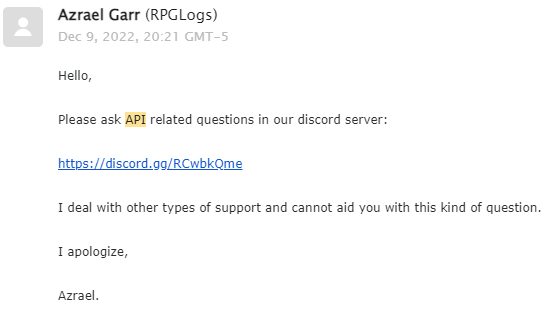
\includegraphics[width=0.5\textwidth]{mail1.PNG}
\caption{Mail received from the support team at \textsc{WarcraftLogs}}
\label{fig:MailSupp}
\end{figure}


\chapter{Schema}

\section{Generic \ttt{Types}}

\underline{\textbf{\ttt{Int}}:}

An integer is a whole number $n\in A\subset\mb{Z}$ where $A$ is finite. \textsc{GraphQL} can handle both 32 and 64 bit int, since \tsc{GraphQL V16}. \ttt{Int} is still just a 32 bit integer even though it could support it. Note that the type \ttt{Int} is a signed 32 bit integer.

\medskip

\textit{note:} There is no reason to use 64 bit integers since neither \tsc{WoW} or \tsc{FF14} uses this.

\medskip

\underline{\textbf{\ttt{String}}:}

A \ttt{String} is a scalar of a list of characters i.e \ttt{"This Is a string example"}. Since \ttt{String} is a scalar, there is theocratically no limits for the length in \tsc{GraphQL}. This hasn't been tested to check wether or not \tsc{WarcraftLogsAPI} support very long strings. Practically there is no need for very long strings.

\medskip

\underline{\textbf{\ttt{Boolean}}:}

a \ttt{Boolean} is either \ttt{true} or \ttt{false}. No further explanation is needed.

\medskip

\underline{\textbf{\ttt{Float}}:}

A \ttt{Float} is a signed double precision floating point value, i.e \ttt{float64} or \ttt{IEEE 754 double-precision binary floating-point format} (\cite{floatsWiki}). 

\medskip

\underline{\textbf{\ttt{Generic.Enum}}:}
A \ttt{Generic.Enum} type doesn't exists within \tsc{GraphQL}. It's up to the developer using \tsc{GraphQL} to implements such types. These can be seen in \cref{sec:Enums}. They don't need string to around them when writing i.e \ttt{dataType: Deaths} where \ttt{Deaths} is of a type \ttt{EventDataType}

\medskip

\underline{\textbf{\ttt{Generic.Pagination}}:}

A \ttt{Pagination} object is an object where some of its data types withing the object is returned as a list.

\smallskip

\textit{Example:} Instead of calling three different players within a guild where these players have type \type{Character} we can just call to the type \type{CharacterPagination} where you give the arguments \ttt{guildID: \type{Int}, limit: \type{Int}, page: \type{Int}}. From here we can get all members of the guild and then from our end remove all unwanted players. This is smart, since we don't need to make three calls but just one call.

\newpage

\section{Overview}

\begin{itemize}[noitemsep,topsep=1pt]
\item[\textbf{Main Call:}] query
	\begin{itemize}[noitemsep,topsep=1pt]
		\item \ttt{characterData: \hyperref[sec:CharacterData]{\type{CharacterData}}}
		\item \ttt{gameData: \hyperref[sec:GameData]{\type{GameData}}}
		\item \ttt{guildData: \hyperref[sec:GuildData]{\type{GuildData}}}
		\item \ttt{progressRaceData: \hyperref[sec:ProgressRaceData]{\type{ProgressRaceData}}}
		\item \ttt{rateLimitData: \hyperref[sec:RateLimitData]{\type{RateLimitData}}}
		\item \ttt{reportData: \hyperref[sec:ReportData]{\type{ReportData}}}
		\item \ttt{userData: \hyperref[sec:UserData]{\type{UserData}}}
		\item \ttt{worldData: \hyperref[sec:WorldData]{\type{WorldData}}}
	\end{itemize}
\end{itemize}

\underline{\textbf{Details:}}

\ttt{query} is the main call and is has type \type{Query}. The outputs of this \type{Query} can by any of the \ttt{Data} types. 

\underline{\textbf{Example}}

\begin{lstlisting}[language=WowAPI]
query{
	characterData{
		//Insert CharacterData calls here
	}
	reportData{
		//Insert ReportData calls here
	}
}
\end{lstlisting}


\newpage

\section{\ttt{CharacterData}}\label{sec:CharacterData}

\begin{itemize}[noitemsep,topsep=1pt]
\item[\ttt{Type}] \ttt{CharacterData}
\begin{itemize}[itemsep=1pt,topsep=1pt]
\item \ttt{character(id: \type{Int}, serverSlug: \type{String}, serverRegion: \type{String}): \hyperref[sec:Character]{\type{Character}}}
\item \ttt{characters(guildID: \type{Int}, limit: \type{Int}, page: \type{Int}): \hyperref[sec:characterpagination]{\type{CharacterPagination}}}
\end{itemize}
\end{itemize}

\underline{\textbf{Details:}}

\textbf{\ttt{character}:}

\begin{table}[h]
	\centering
	\begin{tabular}{ |p{3cm}|p{3cm}|p{3cm}|  }
		\hline
		\multicolumn{3}{|c|}{Input List} \\
		\hline
		Input & Type & Requirement\\
		\hline
		\ttt{id}   & \ttt{Int} & Optional\\
		\ttt{name}& \ttt{String} & Optional\\
		\ttt{serverSlug} & \ttt{String} & Optional\\
		\ttt{serverRegion}    & \ttt{String} & Optional\\
		\hline
		\multicolumn{3}{|c|}{Output Type: \ttt{Character}} \\
		\hline
	\end{tabular}
\end{table}



\smallskip

\textbf{\ttt{characters}:}

\begin{table}[h]
	\centering
	\begin{tabular}{ |p{3cm}|p{3cm}|p{3cm}|  }
		\hline
		\multicolumn{3}{|c|}{Input List} \\
		\hline
		Input & Type & Requirement\\
		\hline
		\ttt{guildID}   & \ttt{Int} & Required\\
		\ttt{limit}& \ttt{Int} & Optional\\
		\ttt{page} & \ttt{Int} & Optional\\
		\hline
		\multicolumn{3}{|c|}{Output Type: \ttt{CharacterPagination}} \\
		\hline
	\end{tabular}
\end{table}

\subsection{\ttt{Character}}\label{sec:Character}

\begin{itemize}[noitemsep,topsep=1pt]
	\item[\ttt{Type}] \ttt{Character}
	\begin{itemize}[itemsep=1pt,topsep=1pt]
		\item \ttt{canonicalID: \type{Int}!}
		\item \ttt{claimed: \type{Boolean}}
		\item \ttt{classID: \type{Int}!}
		\item \ttt{encounterRankings(byBracket: \type{Boolean}, \\className: \type{String}, \\compare: \hyperref[sec:RankingCompareType]{\type{RankingCompareType}}, \\difficulty: \type{Int}, \\encounterID: \type{Int}, \\includeCombatantInfo: \type{Boolean}, \\includePrivateLogs: \type{Boolean}, \\metric: \hyperref[sec:CharacterRankingMetricType]{\type{CharacterRankingMetricType}}, \\partition: \type{Int}, \\role: \hyperref[sec:RoleType]{\type{RoleType}}, \\size: \type{Int}, \\specName: \type{String}, \\timeframe: \hyperref[sec:RankingTimeframeType]{\type{RankingTimeframeType}}): \type{JSON}}
		\item \ttt{faction: \hyperref[sec:GameFaction]{\type{GameFaction}}!}
		\item \ttt{gameData(specID: \type{Int}, forceUpdate: \type{Boolean}): \type{JSON}}
		\item \ttt{guildRank: \type{Int}!}
		\item \ttt{guilds: [\hyperref[sec:Guild]{\type{Guild}}]}
		\item \ttt{hidden: \type{Boolean}!}
		\item \ttt{id: \type{Int}!}
		\item \ttt{level: \type{Int}!}
		\item \ttt{name: \type{String}}
		\item \ttt{recentReports(limit: \type{Int}, page: \type{Int}): \hyperref[sec:reportpagination]{\type{ReportPagination}}}
		\item \ttt{server: \hyperref[sec:Server]{\type{Server}}!}
		\item \ttt{zoneRankings(byBracket: \type{Boolean}, \\className: \type{String}, \\compare: \hyperref[sec:RankingCompareType]{\type{RankingCompareType}}, \\difficulty: \type{Int}, \\includePrivateLogs: \type{Boolean}, \\metric: \hyperref[sec:CharacterRankingMetricType]{\type{CharacterRankingMetricType}}, \\partition: \type{Int}, \\role: \hyperref[sec:RoleType]{\type{RoleType}}, \\size: \type{Int}, \\specName: \type{String}, \\timeframe: \hyperref[sec:RankingTimeframeType]{\type{RankingTimeframeType}}, \\zoneID: \type{Int}): \type{JSON}}
	\end{itemize}
\end{itemize}

\underline{\textbf{Details:}}

\textbf{\ttt{canonicalID}:}

\begin{table}[h]
	\centering
	\begin{tabular}{ |p{3cm}|p{3cm}|p{3cm}|  }
		\hline
		\multicolumn{3}{|c|}{Output Type: \ttt{Int!}} \\
		\hline
	\end{tabular}
\end{table}


\medskip

\textbf{\ttt{claimed}:}

\begin{table}[h]
	\centering
	\begin{tabular}{ |p{3cm}|p{3cm}|p{3cm}|  }
		\hline
		\multicolumn{3}{|c|}{Output Type: \ttt{Boolean}} \\
		\hline
	\end{tabular}
\end{table}

\medskip

\textbf{\ttt{classID}:}

\begin{table}[h]
	\centering
	\begin{tabular}{ |p{3cm}|p{3cm}|p{3cm}|  }
		\hline
		\multicolumn{3}{|c|}{Output Type: \ttt{Int!}} \\
		\hline
	\end{tabular}
\end{table}

\medskip

\newpage

\textbf{\ttt{encounterRankings}:}

\begin{table}[h!]
	\centering
	\begin{tabular}{ |p{4.2cm}|p{6cm}|p{3cm}|  }
		\hline
		\multicolumn{3}{|c|}{Input List} \\
		\hline
		Input & Type & Requirement\\
		\hline
		\ttt{byBracket}   & \ttt{Boolean} & Optional\\
		\ttt{className}& \ttt{String} & Optional\\
		\ttt{compare} & \ttt{RankingCompareType} & Optional\\
		\ttt{difficulty} & \ttt{Int} & Optional\\
		\ttt{encounterID} & \ttt{Int} & Required\\
		\ttt{includeCombatantInfo} & \ttt{Boolean} & Optional\\
		\ttt{includePrivateLogs} & \ttt{Boolean} & Optional\\
		\ttt{metric} & \ttt{CharacterRankingMetricType} & Optional\\
		\ttt{partition} & \ttt{Int} & Optional\\
		\ttt{role} & \ttt{RoleType} & Optional\\
		\ttt{size} & \ttt{Int} & Optional\\
		\ttt{specName} & \ttt{String} & Optional\\
		\ttt{timeframe} & \ttt{RankingTimeframeType} & Optional\\
		\hline
		\multicolumn{3}{|c|}{Output Type: \ttt{JSON}} \\
		\hline
	\end{tabular}
\end{table}

\medskip

\textbf{\ttt{faction}:}

\begin{table}[h]
	\centering
	\begin{tabular}{ |p{3cm}|p{3cm}|p{3cm}|  }
		\hline
		\multicolumn{3}{|c|}{Output Type: \ttt{GameFaction!}} \\
		\hline
	\end{tabular}
\end{table}

\medskip

\textbf{\ttt{gameData}:}

\begin{table}[h]
	\centering
	\begin{tabular}{ |p{3cm}|p{3cm}|p{3cm}|  }
		\hline
		\multicolumn{3}{|c|}{Output Type: \ttt{JSON}} \\
		\hline
	\end{tabular}
\end{table}

\medskip

\textbf{\ttt{guildRank}:}

\begin{table}[h]
	\centering
	\begin{tabular}{ |p{3cm}|p{3cm}|p{3cm}|  }
		\hline
		\multicolumn{3}{|c|}{Output Type: \ttt{Int!}} \\
		\hline
	\end{tabular}
\end{table}

\medskip

\textbf{\ttt{guilds}:}

\begin{table}[h!]
	\centering
	\begin{tabular}{ |p{3cm}|p{3cm}|p{3cm}|  }
		\hline
		\multicolumn{3}{|c|}{Output Type: [\ttt{Guild}]} \\
		\hline
	\end{tabular}
\end{table}

\medskip

\textbf{\ttt{hidden}:}

\begin{table}[h!]
	\centering
	\begin{tabular}{ |p{3cm}|p{3cm}|p{3cm}|  }
		\hline
		\multicolumn{3}{|c|}{Output Type: \ttt{Boolean!}} \\
		\hline
	\end{tabular}
\end{table}

\medskip

\textbf{\ttt{id}:}

\begin{table}[h!]
	\centering
	\begin{tabular}{ |p{3cm}|p{3cm}|p{3cm}|  }
		\hline
		\multicolumn{3}{|c|}{Output Type: \ttt{Int!}} \\
		\hline
	\end{tabular}
\end{table}

\newpage

\textbf{\ttt{level}:}

\begin{table}[h!]
	\centering
	\begin{tabular}{ |p{3cm}|p{3cm}|p{3cm}|  }
		\hline
		\multicolumn{3}{|c|}{Output Type: \ttt{Int!}} \\
		\hline
	\end{tabular}
\end{table}

\medskip

\textbf{\ttt{name}:}

\begin{table}[h!]
	\centering
	\begin{tabular}{ |p{3cm}|p{3cm}|p{3cm}|  }
		\hline
		\multicolumn{3}{|c|}{Output Type: \ttt{String}} \\
		\hline
	\end{tabular}
\end{table}

\medskip

\textbf{\ttt{recentReports}:}

\begin{table}[h!]
	\centering
	\begin{tabular}{ |p{4.2cm}|p{6cm}|p{3cm}|  }
		\hline
		\multicolumn{3}{|c|}{Input List} \\
		\hline
		Input & Type & Requirement\\
		\hline
		\ttt{Limit} & \ttt{Int} & Optional\\
		\ttt{page} & \ttt{Int} & Optional\\
		\hline
		\multicolumn{3}{|c|}{Output Type: \ttt{ReportPagination}} \\
		\hline
	\end{tabular}
\end{table}

\medskip

\textbf{\ttt{server}:}

\begin{table}[h!]
	\centering
	\begin{tabular}{ |p{3cm}|p{3cm}|p{3cm}|  }
		\hline
		\multicolumn{3}{|c|}{Output Type: \ttt{Server!}} \\
		\hline
	\end{tabular}
\end{table}

\medskip

\textbf{\ttt{zoneRankings}:}

\begin{table}[h!]
	\centering
	\begin{tabular}{ |p{4.2cm}|p{6cm}|p{3cm}|  }
		\hline
		\multicolumn{3}{|c|}{Input List} \\
		\hline
		Input & Type & Requirement\\
		\hline
		\ttt{byBracket} & \ttt{Boolean} & Optional\\
		\ttt{className} & \ttt{String} & Optional\\
		\ttt{compare} & \ttt{RankingCompareType} & Optional\\
		\ttt{difficulty} & \ttt{Int} & Optional\\
		\ttt{includePrivateLogs} & \ttt{Boolean} & Optional\\
		\ttt{metric} & \ttt{CharacterRankingMetricType} & Optional\\
		\ttt{partition} & \ttt{Int} & Optional\\
		\ttt{role} & \ttt{RoleType} & Optional\\
		\ttt{size} & \ttt{Int} & Optional\\
		\ttt{specName} & \ttt{String} & Optional\\
		\ttt{timeframe} & \ttt{RankingTimeframeType} & Optional\\
		\ttt{zoneID} & \ttt{Int} & Optional\\
		\hline
		\multicolumn{3}{|c|}{Output Type: \ttt{JSON}} \\
		\hline
	\end{tabular}
\end{table}

\newpage

\subsection{Example}

\begin{lstlisting}[language=WowAPI]
query{
	characterData{
		character(id: 0000, name: "test"){
			claimed
			classID
			hidden
			id
			server{
				id
				name
			}
		}
	}
}
\end{lstlisting}

This query call makes the toplevel call to \ttt{query}. Then after that it chooses the \ttt{characterData} call as it sub call category. Thereafter we then further call  the \ttt{character} sub call category and gives the required arguments. Then we call to get the data \ttt{claimed, classID, hidden, id, server} where \ttt{server} return \ttt{id} and \ttt{name} as it data.  

\newpage

\section{\ttt{GameData}}\label{sec:GameData}

\begin{itemize}[noitemsep,topsep=1pt]
\item[\ttt{Type}] \ttt{GameData}
\begin{itemize}[itemsep=1pt,topsep=1pt]
\item \ttt{abilities(limit: \type{Int}, page: \type{Int}): \hyperref[sec:gameabilitypagination]{\type{GameAbilityPagination}}}
\item \ttt{ability(id: \type{Int}): \hyperref[sec:GameAbility]{\type{GameAbility}}}
\item \ttt{achievement(id: \type{Int}): \hyperref[sec:GameAchievement]{\type{GameAchievement}}}
\item \ttt{achievements(limit: \type{Int}, page: \type{Int}): \hyperref[sec:gameachievementpagination]{\type{GameAchievementPagination}}}
\item \ttt{affix(id: \type{Int}): \hyperref[sec:GameAffix]{\type{GameAffix}}}
\item \ttt{affixes: [\hyperref[sec:GameAffix]{\type{GameAffix}}]}
\item \ttt{class(id: \type{Int}, faction\_id: \type{Int}, zone\_id: \type{Int}): \hyperref[sec:GameClass]{\type{GameClass}}}
\item \ttt{classes(faction\_id: \type{Int}, zone\_id: \type{Int}): [\hyperref[sec:GameClass]{\type{GameClass}}]}
\item \ttt{enchant(id: \type{Int}): \hyperref[sec:GameEnchant]{\type{GameEnchant}}}
\item \ttt{enchants(limit: \type{Int}, page: \type{Int}): \hyperref[sec:gameenchantpagination]{\type{GameEnchantPagination}}}
\item \ttt{factions: [\hyperref[sec:GameFaction]{\type{GameFaction}}]}
\item \ttt{item(id: \type{Int}): \hyperref[sec:GameItem]{\type{GameItem}}}
\item \ttt{item\_set(id: \type{Int}): \hyperref[sec:GameItemSet]{\type{GameItemSet}}}
\item \ttt{item\_sets(limit: \type{Int}, page: \type{Int}): \hyperref[sec:gameitemsetpagination]{\type{GameItemSetPagination}}}
\item \ttt{items(limit: \type{Int}, page: \type{Int}): \hyperref[sec:gameitempagination]{\type{GameItemPagination}}}
\item \ttt{map(id: \type{Int}): \hyperref[sec:GameMap]{\type{GameMap}}}
\item \ttt{maps(limit: \type{Int}, page: \type{Int}): \hyperref[sec:gamemappagination]{\type{GameMapPagination}}}
\item \ttt{npc(id: \type{Int}): \hyperref[sec:GameNPC]{\type{GameNPC}}}
\item \ttt{npcs(limit: \type{Int}, page: \type{Int}): \hyperref[sec:gamenpcpagination]{\type{GameNPCPagination}}}
\item \ttt{zone(id: \type{Int}): \hyperref[sec:GameZone]{\type{GameZone}}}
\item \ttt{zones(limit: \type{Int}, page: \type{Int}): \hyperref[sec:gamezonepagination]{\type{GameZonePagination}}}
\end{itemize}
\end{itemize}

\underline{\textbf{Details:}}

\textbf{abilities:}
\begin{table}[h!]
	\centering
	\begin{tabular}{ |p{4.2cm}|p{6cm}|p{3cm}|  }
		\hline
		\multicolumn{3}{|c|}{Input List} \\
		\hline
		Input & Type & Requirement\\
		\hline
		\ttt{limit} & \ttt{Int} & Optional\\
		\ttt{page} & \ttt{Int} & Optional\\
		\hline
		\multicolumn{3}{|c|}{Output Type: \ttt{GameAbilityPagination}} \\
		\hline
	\end{tabular}
\end{table}

\medskip

\textbf{ability:}

\begin{table}[h!]
	\centering
	\begin{tabular}{ |p{4.2cm}|p{6cm}|p{3cm}|  }
		\hline
		\multicolumn{3}{|c|}{Input List} \\
		\hline
		Input & Type & Requirement\\
		\hline
		\ttt{id} & \ttt{Int} & Required\\
		\hline
		\multicolumn{3}{|c|}{Output Type: \ttt{GameAbility}} \\
		\hline
	\end{tabular}
\end{table}

\newpage

\textbf{achievement:}

\begin{table}[h!]
	\centering
	\begin{tabular}{ |p{4.2cm}|p{6cm}|p{3cm}|  }
		\hline
		\multicolumn{3}{|c|}{Input List} \\
		\hline
		Input & Type & Requirement\\
		\hline
		\ttt{id} & \ttt{Int} & Required\\
		\hline
		\multicolumn{3}{|c|}{Output Type: \ttt{GameAchievement}} \\
		\hline
	\end{tabular}
\end{table}

\medskip

\textbf{achievements:}

\begin{table}[h!]
	\centering
	\begin{tabular}{ |p{4.2cm}|p{6cm}|p{3cm}|  }
		\hline
		\multicolumn{3}{|c|}{Input List} \\
		\hline
		Input & Type & Requirement\\
		\hline
		\ttt{int} & \ttt{Int} & Optional\\
		\ttt{page} & \ttt{Int} & Optional\\
		\hline
		\multicolumn{3}{|c|}{Output Type: \ttt{GameAchievementPagination}} \\
		\hline
	\end{tabular}
\end{table}

\medskip

\textbf{affix:}

\begin{table}[h!]
	\centering
	\begin{tabular}{ |p{4.2cm}|p{6cm}|p{3cm}|  }
		\hline
		\multicolumn{3}{|c|}{Input List} \\
		\hline
		Input & Type & Requirement\\
		\hline
		\ttt{id} & \ttt{Int} & Required\\
		\hline
		\multicolumn{3}{|c|}{Output Type: \ttt{GameAffix}} \\
		\hline
	\end{tabular}
\end{table}

\medskip

\textbf{affixes:}

\begin{table}[h!]
	\centering
	\begin{tabular}{ |p{4.2cm}|p{6cm}|p{3cm}|  }
		\hline
		\multicolumn{3}{|c|}{Output Type: \ttt{[GameAffix]}} \\
		\hline
	\end{tabular}
\end{table}

\medskip

\textbf{class:}

\begin{table}[h!]
	\centering
	\begin{tabular}{ |p{4.2cm}|p{6cm}|p{3cm}|  }
		\hline
		\multicolumn{3}{|c|}{Input List} \\
		\hline
		Input & Type & Requirement\\
		\hline
		\ttt{id} & \ttt{Int} & Required\\
		\ttt{faction\_id} & \ttt{Int} & Optional\\
		\ttt{zone\_id} & \ttt{Int} & Optional\\
		\hline
		\multicolumn{3}{|c|}{Output Type: \ttt{GameClass}} \\
		\hline
	\end{tabular}
\end{table}

\medskip

\textbf{classes:}

\begin{table}[h!]
	\centering
	\begin{tabular}{ |p{4.2cm}|p{6cm}|p{3cm}|  }
		\hline
		\multicolumn{3}{|c|}{Input List} \\
		\hline
		Input & Type & Requirement\\
		\hline
		\ttt{faction\_id} & \ttt{Int} & Optional\\
		\ttt{zone\_id} & \ttt{Int} & Optional\\
		\hline
		\multicolumn{3}{|c|}{Output Type: \ttt{[GameClass]}} \\
		\hline
	\end{tabular}
\end{table}

\newpage

\textbf{enchant:}

\begin{table}[h!]
	\centering
	\begin{tabular}{ |p{4.2cm}|p{6cm}|p{3cm}|  }
		\hline
		\multicolumn{3}{|c|}{Input List} \\
		\hline
		Input & Type & Requirement\\
		\hline
		\ttt{id} & \ttt{Int} & Required\\
		\hline
		\multicolumn{3}{|c|}{Output Type: \ttt{GameEnchant}} \\
		\hline
	\end{tabular}
\end{table}

\medskip

\textbf{enchants:}

\begin{table}[h!]
	\centering
	\begin{tabular}{ |p{4.2cm}|p{6cm}|p{3cm}|  }
		\hline
		\multicolumn{3}{|c|}{Input List} \\
		\hline
		Input & Type & Requirement\\
		\hline
		\ttt{limit} & \ttt{Int} & Optional\\
		\ttt{page} & \ttt{Int} & Optional\\
		\hline
		\multicolumn{3}{|c|}{Output Type: \ttt{GameEnchantPagination}} \\
		\hline
	\end{tabular}
\end{table}

\medskip

\textbf{factions:}

\begin{table}[h!]
	\centering
	\begin{tabular}{ |p{4.2cm}|p{6cm}|p{3cm}|  }
		\hline
		\multicolumn{3}{|c|}{Output Type: \ttt{[GameFaction]}} \\
		\hline
	\end{tabular}
\end{table}

\medskip

\textbf{item:}

\begin{table}[h!]
	\centering
	\begin{tabular}{ |p{4.2cm}|p{6cm}|p{3cm}|  }
		\hline
		\multicolumn{3}{|c|}{Input List} \\
		\hline
		Input & Type & Required\\
		\hline
		\ttt{id} & \ttt{Int} & Requirement\\
		\hline
		\multicolumn{3}{|c|}{Output Type: \ttt{GameItem}} \\
		\hline
	\end{tabular}
\end{table}

\medskip

\textbf{item\_set:}

\begin{table}[h!]
	\centering
	\begin{tabular}{ |p{4.2cm}|p{6cm}|p{3cm}|  }
		\hline
		\multicolumn{3}{|c|}{Input List} \\
		\hline
		Input & Type & Requirement\\
		\hline
		\ttt{id} & \ttt{Int} & Required\\
		\hline
		\multicolumn{3}{|c|}{Output Type: \ttt{GameItemSet}} \\
		\hline
	\end{tabular}
\end{table}

\medskip

\textbf{item\_sets:}

\begin{table}[h!]
	\centering
	\begin{tabular}{ |p{4.2cm}|p{6cm}|p{3cm}|  }
		\hline
		\multicolumn{3}{|c|}{Input List} \\
		\hline
		Input & Type & Requirement\\
		\hline
		\ttt{limit} & \ttt{Int} & Optional\\
		\ttt{page} & \ttt{Int} & Optional\\
		\hline
		\multicolumn{3}{|c|}{Output Type: \ttt{GameItemSetPagination}} \\
		\hline
	\end{tabular}
\end{table}

\newpage

\textbf{items:}

\begin{table}[h!]
	\centering
	\begin{tabular}{ |p{4.2cm}|p{6cm}|p{3cm}|  }
		\hline
		\multicolumn{3}{|c|}{Input List} \\
		\hline
		Input & Type & Requirement\\
		\hline
		\ttt{limit} & \ttt{Int} & Optional\\
		\ttt{page} & \ttt{Int} & Optional\\
		\hline
		\multicolumn{3}{|c|}{Output Type: \ttt{GameItemPagination}} \\
		\hline
	\end{tabular}
\end{table}

\medskip

\textbf{map:}

\begin{table}[h!]
	\centering
	\begin{tabular}{ |p{4.2cm}|p{6cm}|p{3cm}|  }
		\hline
		\multicolumn{3}{|c|}{Input List} \\
		\hline
		Input & Type & Requirement\\
		\hline
		\ttt{id} & \ttt{Int} & Required\\
		\hline
		\multicolumn{3}{|c|}{Output Type: \ttt{GameMap}} \\
		\hline
	\end{tabular}
\end{table}

\medskip

\textbf{maps:}

\begin{table}[h!]
	\centering
	\begin{tabular}{ |p{4.2cm}|p{6cm}|p{3cm}|  }
		\hline
		\multicolumn{3}{|c|}{Input List} \\
		\hline
		Input & Type & Requirement\\
		\hline
		\ttt{limit} & \ttt{Int} & Optional\\
		\ttt{page} & \ttt{Int} & Optional\\
		\hline
		\multicolumn{3}{|c|}{Output Type: \ttt{GameMapPagination}} \\
		\hline
	\end{tabular}
\end{table}

\medskip

\textbf{npc:}

\begin{table}[h!]
	\centering
	\begin{tabular}{ |p{4.2cm}|p{6cm}|p{3cm}|  }
		\hline
		\multicolumn{3}{|c|}{Input List} \\
		\hline
		Input & Type & Requirement\\
		\hline
		\ttt{id} & \ttt{Int} & Required\\
		\hline
		\multicolumn{3}{|c|}{Output Type: \ttt{GameNPC}} \\
		\hline
	\end{tabular}
\end{table}

\medskip

\textbf{npcs:}

\begin{table}[h!]
	\centering
	\begin{tabular}{ |p{4.2cm}|p{6cm}|p{3cm}|  }
		\hline
		\multicolumn{3}{|c|}{Input List} \\
		\hline
		Input & Type & Requirement\\
		\hline
		\ttt{limit} & \ttt{Int} & Optional\\
		\ttt{page} & \ttt{Int} & Optional\\
		\hline
		\multicolumn{3}{|c|}{Output Type: \ttt{GameNPCPagination}} \\
		\hline
	\end{tabular}
\end{table}

\medskip

\textbf{zone:}

\begin{table}[h!]
	\centering
	\begin{tabular}{ |p{4.2cm}|p{6cm}|p{3cm}|  }
		\hline
		\multicolumn{3}{|c|}{Input List} \\
		\hline
		Input & Type & Requirement\\
		\hline
		\ttt{id} & \ttt{Int} & Required\\
		\hline
		\multicolumn{3}{|c|}{Output Type: \ttt{GameZone}} \\
		\hline
	\end{tabular}
\end{table}

\newpage

\textbf{zones:}

\begin{table}[h!]
	\centering
	\begin{tabular}{ |p{4.2cm}|p{6cm}|p{3cm}|  }
		\hline
		\multicolumn{3}{|c|}{Input List} \\
		\hline
		Input & Type & Requirement\\
		\hline
		\ttt{limit} & \ttt{Int} & Optional\\
		\ttt{page} & \ttt{Int} & Optional\\
		\hline
		\multicolumn{3}{|c|}{Output Type: \ttt{GameZonePagination}} \\
		\hline
	\end{tabular}
\end{table}

\subsection{\ttt{GameAbility}}\label{sec:GameAbility}

\begin{itemize}[noitemsep,topsep=1pt]
\item[\ttt{Type}] \ttt{GameAbility}
\begin{itemize}[itemsep=1pt,topsep=1pt]
\item \ttt{id: \type{Int}!}
\item \ttt{icon: \type{String}}
\item \ttt{name: \type{String}}
\end{itemize}
\end{itemize}

\subsection{\ttt{GameAchievement}}\label{sec:GameAchievement}

\begin{itemize}[noitemsep,topsep=1pt]
\item[\ttt{Type}] \ttt{GameAchievement}
\begin{itemize}[itemsep=1pt,topsep=1pt]
\item \ttt{id: \type{Int}!}
\item \ttt{icon: \type{String}}
\item \ttt{name: \type{String}}
\end{itemize}
\end{itemize}

\subsection{\ttt{GameAffix}}\label{sec:GameAffix}

\begin{itemize}[noitemsep,topsep=1pt]
\item[\ttt{Type}] \ttt{GameAffix}
\begin{itemize}[itemsep=1pt,topsep=1pt]
\item \ttt{id: \type{Int}!}
\item \ttt{icon: \type{String}}
\item \ttt{name: \type{String}}
\end{itemize}
\end{itemize}

\subsection{\ttt{GameClass}}\label{sec:GameClass}

\begin{itemize}[noitemsep,topsep=1pt]
\item[\ttt{Type}] \ttt{GameClass}
\begin{itemize}[itemsep=1pt,topsep=1pt]
\item \ttt{id: \type{Int}!}
\item \ttt{name: \type{String}!}
\item \ttt{slug: \type{String}!}
\item \ttt{specs: \hyperref[sec:GameSpec]{\type{GameSpec}}}
\end{itemize}
\end{itemize}

\subsubsection{\ttt{GameSpec}}\label{sec:GameSpec}

\begin{itemize}[noitemsep,topsep=1pt]
\item[\ttt{Type}] \ttt{GameSpec}
\begin{itemize}[itemsep=1pt,topsep=1pt]
\item \ttt{id: \type{Int}!}
\item \ttt{class: \hyperref[sec:GameClass]{\type{GameClass}}}
\item \ttt{name: \type{String}!}
\item \ttt{slug: \type{String}!}
\end{itemize}
\end{itemize}

\subsection{\ttt{GameEnchant}}\label{sec:GameEnchant}

\begin{itemize}[noitemsep,topsep=1pt]
\item[\ttt{Type}] \ttt{GameEnchant}
\begin{itemize}[itemsep=1pt,topsep=1pt]
\item \ttt{id: \type{Int}!}
\item \ttt{name: \type{String}}
\end{itemize}
\end{itemize}

\subsection{\ttt{GameFaction}}\label{sec:GameFaction}

\begin{itemize}[noitemsep,topsep=1pt]
\item[\ttt{Type}] \type{GameFaction}
\begin{itemize}[itemsep=1pt,topsep=1pt]
\item \ttt{id: \type{Int}!}
\item \ttt{name: \type{String}!}
\end{itemize}
\end{itemize}

\subsection{\ttt{GameItem}}\label{sec:GameItem}

\begin{itemize}[noitemsep,topsep=1pt]
\item[\ttt{Type}] \ttt{GameItem}
\begin{itemize}[itemsep=1pt,topsep=1pt]
\item \ttt{id: \type{Int}!}
\item \ttt{icon: \type{String}}
\item \ttt{name: \type{String}}
\end{itemize}
\end{itemize}

\subsection{\ttt{GameItemSet}}\label{sec:GameItemSet}

\begin{itemize}[noitemsep,topsep=1pt]
\item[\ttt{Type}] \ttt{GameItemSet}
\begin{itemize}[itemsep=1pt,topsep=1pt]
\item \ttt{id: \type{Int}!}
\item \ttt{name: \type{String}}
\end{itemize}
\end{itemize}

\subsection{\ttt{GameMap}}\label{sec:GameMap}

\begin{itemize}[noitemsep,topsep=1pt]
\item[\ttt{Type}] \ttt{GameMap}
\begin{itemize}[itemsep=1pt,topsep=1pt]
\item \ttt{id: \type{Int}!}
\item \ttt{name: \type{String}}
\end{itemize}
\end{itemize}

\subsection{\ttt{GameNPC}}\label{sec:GameNPC}

\begin{itemize}[noitemsep,topsep=1pt]
\item[\ttt{Type}] \ttt{GameNPC}
\begin{itemize}[itemsep=1pt,topsep=1pt]
\item \ttt{id: \type{Int}!}
\item \ttt{name: \type{String}}
\end{itemize}
\end{itemize}

\subsection{\ttt{GameZone}}\label{sec:GameZone}

\begin{itemize}[noitemsep,topsep=1pt]
\item[\ttt{Type}] \ttt{GameZone}
\begin{itemize}[itemsep=1pt,topsep=1pt]
\item \ttt{id: \type{Float}!}
\item \ttt{name: \type{String}}
\end{itemize}
\end{itemize}

\subsection{Example}

\begin{lstlisting}[language=WowAPI]
query{
	gameData{
		ability(id: 420){
			name
		}
		factions{
			name
		}
		class(id: 1, faction_id: 0){
			name
			specs{
				id
				name
				slug
			}
		}
	}
}
\end{lstlisting}

This could be a potential query someone would make. Here we get the \ttt{name} of the \ttt{ability} with \ttt{id: 420}, all \ttt{factions} names and the \ttt{name} and \ttt{specs} of the \ttt{class} with \ttt{id:1} and \ttt{faction\_id:0}.
\newpage


%\begin{itemize}[noitemsep,topsep=1pt]
%\item[\ttt{Type}]
%\begin{itemize}[itemsep=1pt,topsep=1pt]
%\item \ttt{}
%\end{itemize}
%\end{itemize}

\section{\ttt{GuildData}}\label{sec:GuildData}

\begin{itemize}[noitemsep,topsep=1pt]
\item[\ttt{Type}] \ttt{GuildData}
\begin{itemize}[itemsep=1pt,topsep=1pt]
\item \ttt{guild(id: \type{Int}, name: \type{String}, serverSlug: \type{String}, serverRegion: \type{String}): \hyperref[sec:Guild]{\type{Guild}}}
\item \ttt{guilds(limit: \type{Int}, page: \type{Int}, \\serverID: \type{Int}, serverSlug: \type{String}, \\serverRegion: \type{String}): \hyperref[sec:guildpagination]{\type{GuildPagination}}}
\end{itemize}
\end{itemize}

\subsection{\ttt{Guild}}\label{sec:Guild}

\begin{itemize}[noitemsep,topsep=1pt]
	\item[\ttt{Type}] \ttt{Guild}
	\begin{itemize}[itemsep=1pt,topsep=1pt]
		\item \ttt{attendance(guildTagId: \type{Int}, limit: \type{Int}, page: \type{Int}, zoneID: \type{Int}): \hyperref[sec:guildattendancepagination]{\type{GuildAttendancePagination}}!}
		\item \ttt{competitionMode: \type{Boolean}!}
		\item \ttt{description: \type{String}!}
		\item \ttt{faction: \hyperref[sec:GameFaction]{\type{GameFaction}}!}
		\item \ttt{id: \type{Int}!}
		\item \ttt{name: \type{String}!}
		\item \ttt{server:\hyperref[sec:Server]{ \type{Server}}!}
		\item \ttt{stealthMode: \type{Boolean}!}
		\item \ttt{tags: [\hyperref[sec:GuildTag]{\type{GuildTag}}]}
		\item \ttt{members(limit: \type{Int}, page: \type{Int}): \hyperref[sec:characterpagination]{\type{CharacterPagination}}!}
		\item \ttt{currentUserRank: \hyperref[sec:GuildRank]{\type{GuildRank}}}
		\item \ttt{zoneRank(zoneID: \type{Int}): \hyperref[sec:GuildZoneRankings]{\type{GuildZoneRankings}}!}
	\end{itemize}
\end{itemize}

\subsubsection{\ttt{GuildTag}}\label{sec:GuildTag}

\begin{itemize}[noitemsep,topsep=1pt]
\item[\ttt{Type}] \ttt{GuildTag}
\begin{itemize}[itemsep=1pt,topsep=1pt]
\item \ttt{id: \type{Int}!}
\item \ttt{guild: \hyperref[sec:Guild]{\type{Guild}}!}
\item \ttt{name: \type{String}!}
\end{itemize}
\end{itemize}

\subsubsection{\ttt{GuildZoneRankings}}\label{sec:GuildZoneRankings}

\begin{itemize}[noitemsep,topsep=1pt]
\item[\ttt{Type}] \ttt{GuildZoneRankings}
\begin{itemize}[itemsep=1pt,topsep=1pt]
\item \ttt{progress(size: \type{Int}): \hyperref[sec:WorldRegionServerRankPositions]{\type{WorldRegionServerRankPositions}}}
\item \ttt{speed(size: \type{Int}, difficulty: \type{Int}): \hyperref[sec:WorldRegionServerRankPositions]{\type{WorldRegionServerRankPositions}}}
\item \ttt{completeRaidSpeed(size: \type{Int}, difficulty: \type{Int}): \hyperref[sec:WorldRegionServerRankPositions]{\type{WorldRegionServerRankPositions}}}
\end{itemize}
\end{itemize}

\subsubsection{\ttt{GuildAttendance}}\label{sec:GuildAttendance}

\begin{itemize}[noitemsep,topsep=1pt]
\item[\ttt{Type}] \ttt{GuildAttendance}
\begin{itemize}[itemsep=1pt, topsep=1pt]
\item \ttt{code: \type{String}!}
\item \ttt{players: [\hyperref[sec:PlayerAttendance]{\type{PlayerAttendance}}]}
\item \ttt{startTime: \type{Float}}
\item \ttt{zone: \hyperref[sec:Zone]{\type{Zone}}}
\end{itemize}
\end{itemize}

\subsubsection{\ttt{PlayerAttendance}}\label{sec:PlayerAttendance}

\begin{itemize}[noitemsep,topsep=1pt]
\item[\ttt{Type}] \ttt{PlayerAttendance}
\begin{itemize}[itemsep=1pt,topsep=1pt]
\item \ttt{name: \type{String}}
\item \ttt{type: \type{String}}
\item \ttt{presence: \type{Int}}
\end{itemize}
\end{itemize}

\subsection{Example}

\newpage




\section{\ttt{ProgressRaceData}}\label{sec:ProgressRaceData}

\begin{itemize}[noitemsep,topsep=1pt]
	\item[\ttt{Type}] \ttt{ProgressRaceData}
	\begin{itemize}[itemsep=1pt,topsep=1pt]
		\item \ttt{progressRace(serverRegion: \type{String}, ServerSubregion: \type{String}, \\serverSlug: \type{String}, zoneID: \type{Int}, \\competitionID: \type{Int}, difficulty: \type{Int}, \\size: \type{Int}, guildID: \type{Int}, \\guildName: \type{String}): \type{JSON}}
		\item \ttt{detailedComposition(competitionID: \type{Int}, guildID: \type{Int}, \\guildName: \type{String}, serverSlug: \type{String}, \\serverRegion: \type{String}, encounterID: \type{Int}, \\difficulty: \type{Int}, size: \type{Int}): \type{JSON}}
	\end{itemize}
\end{itemize}

\underline{\textbf{Details:}}

\textbf{progressRace:}

\begin{table}[h!]
	\centering
	\begin{tabular}{ |p{4.2cm}|p{6cm}|p{3cm}|  }
		\hline
		\multicolumn{3}{|c|}{Input List} \\
		\hline
		Input & Type & Requirement\\
		\hline
		\ttt{serverRegion} & \ttt{String} & Optional\\
		\ttt{serverSubregion} & \ttt{String} & Optional\\
		\ttt{serverSlug} & \ttt{String} & Optional\\
		\ttt{zoneId} & \ttt{Int} & Optional\\
		\ttt{competitionID} & \ttt{Int} & Optional\\
		\ttt{difficulty} & \ttt{Int} & Optional\\
		\ttt{size} & \ttt{Int} & Optional\\
		\ttt{guildID} & \ttt{Int} & Optional\\
		\ttt{guildName} & \ttt{String} & Optional\\
		\hline
		\multicolumn{3}{|c|}{Output Type: \ttt{JSON}} \\
		\hline
	\end{tabular}
\end{table}

\medskip

\textbf{detailedComposition:}

\begin{table}[h!]
	\centering
	\begin{tabular}{ |p{4.2cm}|p{6cm}|p{3cm}|  }
		\hline
		\multicolumn{3}{|c|}{Input List} \\
		\hline
		Input & Type & Requirement\\
		\hline
		\ttt{competitionID} & \ttt{Int} & Optional\\
		\ttt{guildID} & \ttt{Int} & Optional\\
		\ttt{guildName} & \ttt{String} & Optional\\
		\ttt{serverSlug} & \ttt{String} & Optional\\
		\ttt{serverRegion} & \ttt{String} & Optional\\
		\ttt{encounterID} & \ttt{Int} & Optional\\
		\ttt{difficulty} & \ttt{Int} & Optional\\
		\ttt{size} & \ttt{Int} & Optional\\
		\hline
		\multicolumn{3}{|c|}{Output Type: \ttt{JSON}} \\
		\hline
	\end{tabular}
\end{table}

\subsection{Example}

\newpage




\section{\ttt{RateLimitData}}\label{sec:RateLimitData}

\begin{itemize}[noitemsep,topsep=1pt]
\item[\ttt{Type}] \ttt{RateLimitData}
\begin{itemize}[itemsep=1pt,topsep=1pt]
\item \ttt{limitPerHour: \type{Int}!}
\item \ttt{pointSpentThisHour: \type{Float}!}
\item \ttt{pointsResetIn: \type{Int}!}
\end{itemize}
\end{itemize}

\subsection{Example}

\begin{lstlisting}[language=WowAPI]
query{
	RateLimitData{
		limitPrHour
		pointSpentThisHour
		pointsResetIn
	}
}
\end{lstlisting}

This is a full example of what a query for \ttt{RateLimitData} looks like. 

\newpage




\section{\ttt{ReportData}}\label{sec:ReportData}

\begin{itemize} [noitemsep,topsep=1pt]
\item \ttt{reportData}
	\begin{itemize}[noitemsep,topsep=1pt]
		\item \ttt{report(code: \type{String}): \hyperref[sec:Report]{\type{Report}}}
		\item \ttt{reports(endTime: \type{Float}, \\guildID: \type{Int}, \\guildName: \type{String}, \\guildServerSlug: \type{String}, \\guildServerRegion: \type{String}, \\guildTagID: \type{Int}, \\userID: \type{Int}, \\limit: \type{Int}, \\page: \type{Int}, \\startTime: \type{Float}, \\zoneID: \type{Int}, \\gameZoneID: \type{Int}}): \hyperref[sec:reportpagination]{\type{ReportPagination}}
	\end{itemize}
\end{itemize}

\subsection{\ttt{Report}}\label{sec:Report}

\begin{itemize}[noitemsep,topsep=1pt]
	\item \ttt{report}
	\begin{itemize}[itemsep=1pt,topsep=1pt]
		\item \ttt{code: \type{String!}}
		\item \ttt{endTime: \type{Float!}}
		\item \ttt{events(abilityID: \type{Float}, \\dataType: \hyperref[sec:EventDataType]{\type{EventDataType}}, \\death: \type{Int}, \\difficulty: \type{Int}, \\encounterID: \type{Int}, \\endTime: \type{Float}, \\fightsIDs: [\type{Int}], \\ filterExpression: \type{String}, \\hostilityType: \hyperref[sec:HostilityType]{\type{HostilityType}}, \\includeResources: \type{Boolean}, \\killType: \hyperref[sec:KillType]{\type{KillType}}, \\limit: \type{Int}, \\sourceAurasAbsent: \type{String}, \\sourceAurasPresent: \type{String}, \\sourceClass: \type{Int}, \\sourceID: \type{Int},  \\sourceInstanceID: \type{Int}, \\startTime: \type{Float}, \\targetAurasAbsent: \type{String}, \\targetAurasPresent: \type{String}, \\targetClass: \type{String}, \\targetID: \type{Int}, \\targetInstanceID: \type{Int}, \\translate: \type{Boolean}, \\useAbilityIDs: \type{Boolean}, \\useActorIDs: \type{Boolean}, \\viewOptions: \type{Int}, \\wipeCutoff: \type{Int}): \hyperref[sec:reporteventpaginator]{\type{ReportEventPaginator}}}
		\item \ttt{exportedSegments: \type{Int}!}
		\item \ttt{fights(difficulty: \type{Int}, \\encounterID: \type{Int}, \\fightIDs: [\type{Int}], \\killType: \hyperref[sec:KillType]{\type{KillType}}, \\Translate: \type{Boolean}): [\type{ReportFight}]}
		\item \ttt{graph(abilityID: \type{Float}, \\dataType: \hyperref[sec:GraphDataType]{\type{GraphDataType}}, \\death: \type{Int}, \\difficulty: \type{Int}, \\encounterID: \type{Int}, \\endTime: \type{Float}, \\fightsIDs: [\type{Int}], \\ filterExpression: \type{String}, \\hostilityType: \hyperref[sec:HostilityType]{\type{HostilityType}}, \\killType: \hyperref[sec:KillType]{\type{KillType}}, \\sourceAurasAbsent: \type{String}, \\sourceAurasPresent: \type{String}, \\sourceClass: \type{Int}, \\sourceID: \type{Int}, \\sourceInstanceID: \type{Int}, \\startTime: \type{Float}, \\targetAurasAbsent: \type{String}, \\targetAurasPresent: \type{String}, \\targetClass: \type{String}, \\targetID: \type{Int}, \\targetInstanceID: \type{Int}, \\translate: \type{Boolean}, \\viewOptions: \type{Int}, \\viewBy: \hyperref[sec:ViewType]{\type{ViewType}}, \\wipeCutoff: \type{Int}): \type{JSON}}
		\item \ttt{guild: \type{Guild}}
		\item \ttt{guildTag: \type{GuildTag}}
		\item \ttt{owner: \hyperref[sec:User]{\type{User}}}
		\item \ttt{masterData(translate: \type{Boolean}): \type{ReportMasterData}}
		\item \ttt{playerDetails(difficulty: \type{Int}, \\encounterID: \type{Int}, \\endTime: \type{Float}, \\fightIDs: [\type{Int}], \\killType: \hyperref[sec:KillType]{\type{KillType}}, \\startTime: \type{Float}, \\translate: \type{Boolean}): \type{JSON}}
		\item \ttt{rankedCharacters: [\hyperref[sec:Character]{\type{Character}}]}
		\item \ttt{rankings(compare: \hyperref[sec:RankingCompareType]{\type{RankingCompareType}}, \\difficulty: \type{Int}, \\encounterID: \type{Int}, \\fightIDs: [\type{Int}], \\playerMetric: \hyperref[sec:ReportRankingMetricType]{\type{ReportRankingMetricType}}, \\timeframe: \hyperref[sec:RankingTimeframeType]{\type{RankingTimeframeType}}): \type{JSON}}
		\item \ttt{region: \type{Region}}
		\item \ttt{revision: \type{Int}!}
		\item \ttt{segments: \type{Int}!}
		\item \ttt{startTime: \type{Float}!}
		\item \ttt{table(abilityID: \type{Float}, \\dataType: \hyperref[sec:TableDataType]{\type{TableDataType}}, \\death: \type{Int}, \\difficulty: \type{Int}, \\encounterID: \type{Int}, \\endTime: \type{Float}, \\fightIDs: [\type{Int}], \\filterExpression: \type{String}, \\hostilityType: \hyperref[sec:HostilityType]{\type{HostilityType}}, \\killType: \hyperref[sec:KillType]{\type{KillType}}, \\sourceAurasAbsent: \type{String}, \\sourceAurasPresent: \type{String}, \\sourceClass: \type{String}, \\sourceID: \type{Int}, \\sourceInstanceID: \type{Int}, \\startTime: \type{Float}, \\targetAurasAbsent: \type{String}, \\target AurasPresent: \type{String}, \\targetClass: \type{String}, \\targetID: \type{Int}, \\targetInstanceID: \type{Int}, \\translate: \type{Boolean}, \\viewOptions: \type{Int}, \\viewBy: \hyperref[sec:ViewType]{\type{ViewType}}, \\wipeCutoff: \type{Int}): \type{JSON}}
		\item \ttt{title: \type{String}!}
		\item \ttt{visibility: \type{String}!}
		\item \ttt{zone: \hyperref[sec:Zone]{\type{Zone}}}
		\item \ttt{archiveStatus: \type{ReportArchiveStatus}}
\end{itemize}
\end{itemize}


\subsubsection{ReportFight}\label{sec:ReportFight}

\begin{itemize}[noitemsep, topsep=1pt]
\item \ttt{fights}
\begin{itemize}[itemsep=1pt, topsep=1pt]
\item \ttt{averageItemLevel: \type{Float}}
\item \ttt{bossPercentage: \type{Float}}
\item \ttt{boundingBox: \type{ReportMapBoundingBox}}
\item \ttt{classicSeasonID: \type{Int}}
\item \ttt{completeRaid: \type{Boolean}!}
\item \ttt{difficulty: \type{Int}}
\item \ttt{dungeonPulls: [\type{ReportDungeonPull}]}
\item \ttt{encounterID: \type{Int}!}
\item \ttt{endTime: \type{Float}!}
\item \ttt{enemyNPCs: [\type{ReportFightNPC}]}
\item \ttt{enemyPets: [\type{ReportFightNPC}]}
\item \ttt{enemyPlayers: [\type{Int}]}
\item \ttt{fightpercentage: \type{Float}}
\item \ttt{friendlyNPCs: [\type{ReportFightNPC}]}
\item \ttt{friendlyPets: [\type{ReportFightNPC}]}
\item \ttt{friendlyPlayers: [\type{Int}]}
\item \ttt{gameZone: \type{GameZone}}
\item \ttt{hardModeLevel: \type{Int}}
\item \ttt{id: \type{Int}!}
\item \ttt{inProgress: \type{Boolean}}
\item \ttt{keystoneAffixed: [\type{Int}]}
\item \ttt{keystoneBonus: \type{Int}}
\item \ttt{keystoneLevel: \type{Int}}
\item \ttt{keystoneTime: \type{Int}}
\item \ttt{kill: \type{Boolean}}
\item \ttt{lastPhase: \type{Int}}
\item \ttt{lastPhaseIsIntermission: \type{Boolean}}
\item \ttt{layer: \type{Int}}
\item \ttt{maps: [\type{ReportMap}]}
\item \ttt{name: \type{String}!}
\item \ttt{rating: \type{Int}}
\item \ttt{size: \type{Int}}
\item \ttt{startTime: \type{Float}!}
\item \ttt{talentImportCode(actorID: \type{Int}!): \type{String}}
\item \ttt{wipeCalledTime: \type{Float}}
\end{itemize}
\end{itemize}

\subsubsection{ReportMasterData}\label{sec:ReportMasterData}

\begin{itemize}[noitemsep,topsep=1pt]
\item \ttt{masterData}
\begin{itemize}[itemsep=1pt, topsep=1pt]
\item \ttt{logVersion: \type{Int}!}
\item \ttt{gameVersion: \type{Int}}
\item \ttt{lang: \type{String}}
\item \ttt{abilities: [\type{ReportAbility}]}
\item \ttt{actors(type: \type{String}, \\subType: \type{String}): [\type{ReportActor}]}
\end{itemize}
\end{itemize}

\subsubsection{\ttt{ReportAbility}}\label{sec:ReportAbility}

\begin{itemize}[noitemsep,topsep=1pt]
\item \ttt{abilities}
\begin{itemize}[itemsep=1pt, topsep=1pt]
\item \ttt{gameID: \type{Float}}
\item \ttt{icon: \type{String}}
\item \ttt{name: \type{String}}
\item \ttt{type: \type{String}}
\end{itemize}
\end{itemize}


\subsubsection{\ttt{ReportActor}}\label{sec:ReportActor}

\begin{itemize}[noitemsep,topsep=1pt]
\item \ttt{actors}
\begin{itemize}[itemsep=1pt,topsep=1pt]
\item \ttt{gameID: \type{Float}}
\item \ttt{icon: \type{String}}
\item \ttt{id: \type{Int}}
\item \ttt{name: \type{String}}
\item \ttt{petOwner: \type{Int}}
\item \ttt{server: \type{String}}
\item \ttt{subType: \type{String}}
\item \ttt{type: \type{String}}
\end{itemize}
\end{itemize}

\subsubsection{ReportArchiveStatus}\label{ReportArchiveStatus}


\subsection{Example}

\newpage

\section{\ttt{UserData}}\label{sec:UserData}

\begin{itemize}[noitemsep,topsep=1pt]
\item[\ttt{Type}] \ttt{UserData}
\begin{itemize}[itemsep=1pt,topsep=1pt]
\item \ttt{user(id: \type{Int}): \hyperref[sec:User]{\type{User}}}
\item \ttt{currentUser: \hyperref[sec:User]{\type{User}}}
\end{itemize}
\end{itemize}

\subsection{\ttt{User}}\label{sec:User}

\begin{itemize}[noitemsep,topsep=1pt]
\item[\ttt{Type}] User
\begin{itemize}[itemsep=1pt,topsep=1pt]
\item \ttt{id: \type{Int}!}
\item \ttt{name: \type{String}!}
\item \ttt{guilds: [\type{Guild}]}
\item \ttt{characters: [\hyperref[sec:Character]{\type{Character}}]}
\item \ttt{battleTag: \type{String}}
\end{itemize}
\end{itemize}

\subsection{Example}

\newpage




\section{\ttt{WorldData}}\label{sec:WorldData}

\begin{itemize}[noitemsep,topsep=1pt]
\item \ttt{worldData}
\begin{itemize}[itemsep=1pt,topsep=1pt]
\item \ttt{ecounter(id: \type{Int}): \hyperref[sec:Encounter]{\type{Encounter}}}
\item \ttt{expansion(id: \type{int}): \hyperref[sec:Expansion]{\type{Expansion}}}
\item \ttt{expansions: [\hyperref[sec:Expansion]{\type{Expansion}}]}
\item \ttt{region(id: \type{Int}): \hyperref[sec:Region]{\type{Region}}}
\item \ttt{region: [\hyperref[sec:Region]{\type{Region}}]}
\item \ttt{server(id: \type{Int},\\region: \type{String},\\slug: \type{String}): \hyperref[sec:Server]{\type{Server}}}
\item \ttt{subregion(id: \type{Int}): \hyperref[sec:Subregion]{\type{Subregion}}}
\item \ttt{zone(id: \type{Int}): \hyperref[sec:Zone]{\type{Zone}}}
\item \ttt{zones(expansion\_id: \type{Int}): [\hyperref[sec:Zone]{\type{Zone}}]}
\end{itemize}
\end{itemize}

\subsection{\ttt{Encounter}}\label{sec:Encounter}

\begin{itemize}[noitemsep,topsep=1pt]
	\item[\ttt{Type}] \ttt{Encounter}
	\begin{itemize}[itemsep=1pt,topsep=1pt]
		\item \ttt{id: \type{Int}!}
		\item \ttt{name: \type{String}!}
		\item \ttt{characterRankings(bracket: \type{Int}, \\difficulty: \type{Int}, \\filter: \type{String}, \\page: \type{Int}, \\partition: \type{Int}, \\serverRegion: \type{String}, \\serverSlug: \type{String}, \\size: \type{Int}, \\leaderboard: \hyperref[sec:LeaderboardRank]{\type{LeaderboardRank}}, \\hardModeLevel: \hyperref[sec:HardModeLevelRankFilter]{\type{HardModeLevelRankFilter}}, \\metric: \hyperref[sec:CharacterRankingMetricType]{\type{CharacterRankingMetricType}}, \\includeCombatInfo: \type{Boolean}, \\className: \type{String}, \\specName: \type{String}, \\externalBuffs: \hyperref[sec:ExternalBuffRankFilter]{\type{ExternalBuffRankFilter}}, \\covenantID: \type{Int}, \\soulbindID: \type{Int}): \type{JSON}}
		\item \ttt{fightRankings(bracket: \type{Int}, \\difficulty: \type{Int}, \\filter: \type{String}, \\page: \type{String}, \\partition: \type{Int}, \\serverRegion: \type{String}, \\serverSlug: \type{String}, \\size: \type{Int}, \\leaderboard: \hyperref[sec:LeaderboardRank]{\type{LeaderboardRank}}, \\hardModeLevel: \hyperref[sec:HardModeLevelRankFilter]{\type{HardModeLevelRankFilter}}, \\metric: \hyperref[sec:FightRankingMetricType]{\type{FightRankingMetricType}}): \type{JSON}}
		\item \ttt{zone: \hyperref[sec:Zone]{\type{Zone}}!}
		\item \ttt{journalID: \type{Int}!}
	\end{itemize}
\end{itemize}

\subsection{\ttt{Expansion}}\label{sec:Expansion}

\begin{itemize}[noitemsep,topsep=1pt]
\item[\ttt{Type}] \ttt{Expansion}
\begin{itemize}[itemsep=1pt,topsep=1pt]
\item \ttt{id: \type{Int}!}
\item \ttt{name: \type{String}!}
\item \ttt{zones: [\hyperref[sec:Zone]{\type{Zone}}]}
\end{itemize}
\end{itemize}
\subsection{\ttt{Region}}\label{sec:Region}

\begin{itemize}[noitemsep,topsep=1pt]
\item[\ttt{Type}] \ttt{Region}
\begin{itemize}[itemsep=1pt,topsep=1pt]
\item \ttt{id: \type{Int}!}
\item \ttt{compactName: \type{String}!}
\item \ttt{name: \type{String}!}
\item \ttt{slug: \type{String}!}
\item \ttt{subregions: [\hyperref[sec:Subregion]{\type{Subregion}}]}
\item \ttt{servers(limit: \type{Int}, page: \type{Int}): \hyperref[sec:serverpagination]{\type{ServerPagination}}}
\end{itemize}
\end{itemize}

\subsection{\ttt{Server}}\label{sec:Server}

%\hyperref[]{

\begin{itemize}[noitemsep,topsep=1pt]
\item[\ttt{Type}] \ttt{Server}
\begin{itemize}[itemsep=1pt,topsep=1pt]
\item \ttt{id: \type{Int}!}
\item \ttt{name: \type{String}!}
\item \ttt{normalizedName: \type{String}!}
\item \ttt{slug: \type{String}!}
\item \ttt{region: \hyperref[sec:Region]{\type{Region}}!}
\item \ttt{subregion: \hyperref[sec:Subregion]{\type{Subregion}}!}
\item \ttt{guilds(limit: \type{Int}, page: \type{Int}): \hyperref[sec:guildpagination]{\type{GuildPagination}}}
\item \ttt{characters(limit: \type{Int}, page: \type{Int}): \hyperref[sec:characterpagination]{\type{CharacterPagination}}}
\end{itemize}
\end{itemize}

\subsection{\ttt{Subregion}}\label{sec:Subregion}

\begin{itemize}[noitemsep,topsep=1pt]
\item[\ttt{Type}] \ttt{Subregion}
\begin{itemize}[itemsep=1pt,topsep=1pt]
\item \ttt{id: \type{Int}!}
\item \ttt{name: \type{String}!}
\item \ttt{region: \type{Region}!}
\item \ttt{servers(limit: \type{Int}, page: \type{Int}): \hyperref[sec:serverpagination]{\type{ServerPagination}}}
\end{itemize}
\end{itemize}


\subsection{\ttt{Zone}}\label{sec:Zone}

\begin{itemize}[noitemsep,topsep=1pt]
\item[\ttt{Type}] \ttt{Zone}
\begin{itemize}[itemsep=1pt,topsep=1pt]
\item \ttt{id: \type{Int}!}
\item \ttt{brackets: \hyperref[sec:Bracket]{\type{Bracket}}}
\item \ttt{difficulties: [\type{Difficulty}]}
\item \ttt{encounters: [\hyperref[sec:Encounter]{\type{Encounter}}]}
\item \ttt{expansion: \hyperref[sec:Expansion]{\type{Expansion}}!}
\item \ttt{frozen: \type{Boolean}!}
\item \ttt{name: \type{String}!}
\item \ttt{partitions: [\hyperref[sec:Partition]{\type{Partition}}]}
\end{itemize}
\end{itemize}

\subsubsection{\ttt{Bracket}}\label{sec:Bracket}
\begin{itemize}[noitemsep,topsep=1pt]
\item \ttt{brackets}
\begin{itemize}[itemsep=1pt,topsep=1pt]
\item \ttt{min: \type{Float}!}
\item \ttt{max: \type{Float}!}
\item \ttt{bucket: \type{Float}}
\item \ttt{type: \type{String}}
\end{itemize}
\end{itemize}

\subsubsection{\ttt{Partition}}\label{sec:Partition}
\begin{itemize}[noitemsep,topsep=1pt]
\item \ttt{partitions}
\begin{itemize}[itemsep=1pt,topsep=1pt]
\item \ttt{id: \type{Int}!}
\item \ttt{name: \type{String}!}
\item \ttt{compactName: \type{String}!}
\item \ttt{default: \type{Boolean}!}
\end{itemize}
\end{itemize}

\subsection{Example}

\newpage

%--------------------------------------------------------- Schema Pagination Objects ---------------------------------------------------------

\section{\ttt{Pagination Objects}}

\subsection{\ttt{CharacterPagination}}\label{sec:characterpagination}

\begin{itemize}[noitemsep,topsep=1pt]
\item[\ttt{Type}] \ttt{CharacterPagination}
\begin{itemize}[itemsep=1pt,topsep=1pt]
\item \ttt{data: [\hyperref[sec:Character]{\type{Character}}]}
\item \ttt{total: \type{Int}!}
\item \ttt{per\_page: \type{Int}!}
\item \ttt{current\_page: \type{Int}!}
\item \ttt{from: \type{Int}}
\item \ttt{to: \type{Int}}
\item \ttt{last\_page: \type{Int}!}
\item \ttt{has\_more\_pages: \type{Boolean}!}
\end{itemize}
\end{itemize}

\subsection{\ttt{GameAchievementPagination}}\label{sec:gameachievementpagination}

\begin{itemize}[noitemsep,topsep=1pt]
\item[\ttt{Type}] \ttt{GameAchievementPagination}
\begin{itemize}[itemsep=1pt,topsep=1pt]
\item \ttt{data: [\hyperref[sec:GameAchievement]{\type{GameAchievement}}]}
\item \ttt{total: \type{Int}!}
\item \ttt{per\_page: \type{Int}!}
\item \ttt{current\_page: \type{Int}!}
\item \ttt{from: \type{Int}}
\item \ttt{to: \type{Int}}
\item \ttt{last\_page: \type{Int}!}
\item \ttt{has\_more\_pages: \type{Boolean}!}
\end{itemize}
\end{itemize}

\subsection{\ttt{GameAbilityPagination}}\label{sec:gameabilitypagination}

\begin{itemize}[noitemsep,topsep=1pt]
\item[\ttt{Type}] \ttt{GameAbilityPagination}
\begin{itemize}[itemsep=1pt,topsep=1pt]
\item \ttt{data: [\hyperref[sec:GameAbility]{\type{GameAbility}}]}
\item \ttt{total: \type{Int}!}
\item \ttt{per\_page: \type{Int}!}
\item \ttt{current\_page: \type{Int}!}
\item \ttt{from: \type{Int}}
\item \ttt{to: \type{Int}}
\item \ttt{last\_page: \type{Int}!}
\item \ttt{has\_more\_pages: \type{Boolean}!}
\end{itemize}
\end{itemize}

\subsection{\ttt{GameEnchantPagination}}\label{sec:gameenchantpagination}

\begin{itemize}[noitemsep,topsep=1pt]
\item[\ttt{Type}] \ttt{GameEnchantPagination}
\begin{itemize}[itemsep=1pt,topsep=1pt]
\item \ttt{data: [\hyperref[sec:GameEnchant]{\type{GameEnchant}}]}
\item \ttt{total: \type{Int}!}
\item \ttt{per\_page: \type{Int}!}
\item \ttt{current\_page: \type{Int}!}
\item \ttt{from: \type{Int}}
\item \ttt{to: \type{Int}}
\item \ttt{last\_page: \type{Int}!}
\item \ttt{has\_more\_pages: \type{Boolean}!}
\end{itemize}
\end{itemize}

\subsection{\ttt{GameItemPagination}}\label{sec:gameitempagination}

\begin{itemize}[noitemsep,topsep=1pt]
\item[\ttt{Type}] \ttt{GameItemPagination}
\begin{itemize}[itemsep=1pt,topsep=1pt]
\item \ttt{data: [\hyperref[sec:GameItem]{\type{GameItem}}]}
\item \ttt{total: \type{Int}!}
\item \ttt{per\_page: \type{Int}!}
\item \ttt{current\_page: \type{Int}!}
\item \ttt{from: \type{Int}}
\item \ttt{to: \type{Int}}
\item \ttt{last\_page: \type{Int}!}
\item \ttt{has\_more\_pages: \type{Boolean}!}
\end{itemize}
\end{itemize}

\subsection{\ttt{GameItemSetPagination}}\label{sec:gameitemsetpagination}

\begin{itemize}[noitemsep,topsep=1pt]
\item[\ttt{Type}] \ttt{GameItemSetPagination}
\begin{itemize}[itemsep=1pt,topsep=1pt]
\item \ttt{data: [\hyperref[sec:GameItemSet]{\type{GameItemSet}}]}
\item \ttt{total: \type{Int}!}
\item \ttt{per\_page: \type{Int}!}
\item \ttt{current\_page: \type{Int}!}
\item \ttt{from: \type{Int}}
\item \ttt{to: \type{Int}}
\item \ttt{last\_page: \type{Int}!}
\item \ttt{has\_more\_pages: \type{Boolean}!}
\end{itemize}
\end{itemize}

\subsection{\ttt{GameMapPagination}}\label{sec:gamemappagination}

\begin{itemize}[noitemsep,topsep=1pt]
\item[\ttt{Type}] \ttt{GameMapPagination}
\begin{itemize}[itemsep=1pt,topsep=1pt]
\item \ttt{data: [\hyperref[sec:GameMap]{\type{GameMap}}]}
\item \ttt{total: \type{Int}!}
\item \ttt{per\_page: \type{Int}!}
\item \ttt{current\_page: \type{Int}!}
\item \ttt{from: \type{Int}}
\item \ttt{to: \type{Int}}
\item \ttt{last\_page: \type{Int}!}
\item \ttt{has\_more\_pages: \type{Boolean}!}
\end{itemize}
\end{itemize}

\subsection{\ttt{GameNPCPagination}}\label{sec:gamenpcpagination}

\begin{itemize}[noitemsep,topsep=1pt]
\item[\ttt{Type}] \ttt{GameNPCPagination}
\begin{itemize}[itemsep=1pt,topsep=1pt]
\item \ttt{data: [\hyperref[sec:GameNPC]{\type{GameNPC}}]}
\item \ttt{total: \type{Int}!}
\item \ttt{per\_page: \type{Int}!}
\item \ttt{current\_page: \type{Int}!}
\item \ttt{from: \type{Int}}
\item \ttt{to: \type{Int}}
\item \ttt{last\_page: \type{Int}!}
\item \ttt{has\_more\_pages: \type{Boolean}!}
\end{itemize}
\end{itemize}

\subsection{\ttt{GameZonePagination}}\label{sec:gamezonepagination}

\begin{itemize}[noitemsep,topsep=1pt]
\item[\ttt{Type}] \ttt{GameZonePagination}
\begin{itemize}[itemsep=1pt,topsep=1pt]
\item \ttt{data: [\hyperref[sec:GameZone]{\type{GameZone}}]}
\item \ttt{total: \type{Int}!}
\item \ttt{per\_page: \type{Int}!}
\item \ttt{current\_page: \type{Int}!}
\item \ttt{from: \type{Int}}
\item \ttt{to: \type{Int}}
\item \ttt{last\_page: \type{Int}!}
\item \ttt{has\_more\_pages: \type{Boolean}!}
\end{itemize}
\end{itemize}

\subsection{\ttt{GuildAttendancePagination}}\label{sec:guildattendancepagination}

\begin{itemize}[noitemsep,topsep=1pt]
\item[\ttt{Type}] \ttt{GuildAttendancePagination}
\begin{itemize}[itemsep=1pt,topsep=1pt]
\item \ttt{data: [\hyperref[sec:GuildAttendance]{\type{GuildAttendance}}]}
\item \ttt{total: \type{Int}!}
\item \ttt{per\_page: \type{Int}!}
\item \ttt{current\_page: \type{Int}!}
\item \ttt{from: \type{Int}}
\item \ttt{to: \type{Int}}
\item \ttt{last\_page: \type{Int}!}
\item \ttt{has\_more\_pages: \type{Boolean}!}
\end{itemize}
\end{itemize}

\subsection{\ttt{GuildPagination}}\label{sec:guildpagination}

\begin{itemize}[noitemsep,topsep=1pt]
\item[\ttt{Type}] \ttt{GuildPagination}
\begin{itemize}[itemsep=1pt,topsep=1pt]
\item \ttt{data: [\hyperref[sec:Guild]{\type{Guild}}]}
\item \ttt{total: \type{Int}!}
\item \ttt{per\_page: \type{Int}!}
\item \ttt{current\_page: \type{Int}!}
\item \ttt{from: \type{Int}}
\item \ttt{to: \type{Int}}
\item \ttt{last\_page: \type{Int}!}
\item \ttt{has\_more\_pages: \type{Boolean}!}
\end{itemize}
\end{itemize}

\subsection{\ttt{ReportEventPaginator}}\label{sec:reporteventpaginator}

\begin{itemize}[noitemsep,topsep=1pt]
\item[\ttt{Type}] \ttt{ReportEventPaginator}
\begin{itemize}[itemsep=1pt,topsep=1pt]
\item \ttt{data: \type{JSON}}
\item \ttt{nextPageTimestamp: \type{Float}}
\end{itemize}
\end{itemize}

\subsection{\ttt{ReportPagination}}\label{sec:reportpagination}

\begin{itemize}[noitemsep,topsep=1pt]
\item[\ttt{Type}] \ttt{ReportPagination}
\begin{itemize}[itemsep=1pt,topsep=1pt]
\item \ttt{data: [\hyperref[sec:Report]{\type{Report}}]}
\item \ttt{total: \type{Int}!}
\item \ttt{per\_page: \type{Int}!}
\item \ttt{current\_page: \type{Int}!}
\item \ttt{from: \type{Int}}
\item \ttt{to: \type{Int}}
\item \ttt{last\_page: \type{Int}!}
\item \ttt{has\_more\_pages: \type{Boolean}!}
\end{itemize}
\end{itemize}

\subsection{\ttt{ServerPagination}} \label{sec:serverpagination}

\begin{itemize}[noitemsep,topsep=1pt]
\item[\ttt{Type}] \ttt{ServerPagination}
\begin{itemize}[itemsep=1pt,topsep=1pt]
\item \ttt{data: [\hyperref[sec:Server]{\type{Server}}]}
\item \ttt{total: \type{Int}!}
\item \ttt{per\_page: \type{Int}!}
\item \ttt{current\_page: \type{Int}!}
\item \ttt{from: \type{Int}}
\item \ttt{to: \type{Int}}
\item \ttt{last\_page: \type{Int}!}
\item \ttt{has\_more\_pages: \type{Boolean}!}
\end{itemize}
\end{itemize}

\newpage

%--------------------------------------------------------- Schema Enums ---------------------------------------------------------

\section{Important \ttt{Types}/\ttt{Enums}}\label{sec:Enums}

\subsection{\ttt{CharacterRankingMetricType}}\label{sec:CharacterRankingMetricType}
\begin{itemize}[noitemsep,topsep=1pt]
\item[\textcolor{blue}{enum}] \ttt{CharacterRankingMetricType}
\begin{itemize}[itemsep=1pt,topsep=1pt]
\item \ttt{bossdps}
\item \ttt{default}
\item \ttt{dps}
\item \ttt{hps}
\item \ttt{krsi}
\item \ttt{playerscore}
\item \ttt{playerspeed}
\item \ttt{tankhps}
\item \ttt{wdps}
\end{itemize}
\end{itemize}


\subsection{\ttt{EventDataType}}\label{sec:EventDataType}
\begin{itemize}[noitemsep,topsep=1pt]
\item[\textcolor{blue}{enum}] \ttt{EventDataType}
\begin{itemize}[itemsep=1pt,topsep=1pt]
\item \ttt{All}
\item \ttt{Buffs}
\item \ttt{Casts}
\item \ttt{CombatantInfo}
\item \ttt{DamageDone}
\item \ttt{DamageTaken}
\item \ttt{Deaths}
\item \ttt{Debuffs}
\item \ttt{Dispels}
\item \ttt{Healing}
\item \ttt{Interrupts}
\item \ttt{Resources}
\item \ttt{Summons}
\item \ttt{Threat}
\end{itemize}
\end{itemize}


\subsection{\ttt{ExternalBuffRankFilter}}\label{sec:ExternalBuffRankFilter}
\begin{itemize}[noitemsep,topsep=1pt]
\item[\textcolor{blue}{enum}] \ttt{ExternalBuffRankFilter}
\begin{itemize}[itemsep=1pt,topsep=1pt]
\item \ttt{Any}
\item \ttt{Require}
\item \ttt{Exclude}
\end{itemize}
\end{itemize}


\subsection{\ttt{FightRankingMetricType}}\label{sec:FightRankingMetricType}
\begin{itemize}[noitemsep,topsep=1pt]
\item[\textcolor{blue}{enum}] \ttt{FightRankingMetricType}
\begin{itemize}[itemsep=1pt,topsep=1pt]
\item \ttt{default}
\item \ttt{execution}
\item \ttt{feats}
\item \ttt{score}
\item \ttt{speed}
\item \ttt{progress}
\end{itemize}
\end{itemize}


\subsection{\ttt{GraphDataType}}\label{sec:GraphDataType}
\begin{itemize}[noitemsep,topsep=1pt]
\item[\textcolor{blue}{enum}] \ttt{GraphDataType}
\begin{itemize}[itemsep=1pt,topsep=1pt]
\item \ttt{Summary}
\item \ttt{Buffs}
\item \ttt{Casts}
\item \ttt{DamageDone}
\item \ttt{DamageTaken}
\item \ttt{Deaths}
\item \ttt{Debuffs}
\item \ttt{Dispels}
\item \ttt{Healing}
\item \ttt{Interrupts}
\item \ttt{Resources}
\item \ttt{Summons}
\item \ttt{Survivability}
\item \ttt{Threat}
\end{itemize}
\end{itemize}


\subsection{\ttt{GuildRank}}\label{sec:GuildRank}
\begin{itemize}[noitemsep,topsep=1pt]
\item[\textcolor{blue}{enum}] \ttt{GuildRank}
\begin{itemize}[itemsep=1pt,topsep=1pt]
\item \ttt{NonMember}
\item \ttt{Applicant}
\item \ttt{Recruit}
\item \ttt{Member}
\item \ttt{Officer}
\item \ttt{GuildMaster}
\end{itemize}
\end{itemize}


\subsection{\ttt{HardModeLevelRankFilter}}\label{sec:HardModeLevelRankFilter}
\begin{itemize}[noitemsep,topsep=1pt]
\item[\textcolor{blue}{enum}] \ttt{HardModeLevelRankFilter}
\begin{itemize}[itemsep=1pt,topsep=1pt]
\item \ttt{Any}
\item \ttt{Highest}
\item \ttt{NormalMode}
\item \ttt{Level0}
\item \ttt{Level1}
\item \ttt{Level2}
\item \ttt{Level3}
\item \ttt{Level4}
\end{itemize}
\end{itemize}


\subsection{\ttt{HostilityType}}\label{sec:HostilityType}
\begin{itemize}[noitemsep,topsep=1pt]
\item[\textcolor{blue}{enum}] \ttt{HostilityType}
\begin{itemize}[itemsep=1pt,topsep=1pt]
\item \ttt{Friendlies}
\item \ttt{Enemies}
\end{itemize}
\end{itemize}


\subsection{\ttt{KillType}}\label{sec:KillType}
\begin{itemize}[noitemsep,topsep=1pt]
\item[\textcolor{blue}{enum}] \ttt{KillType}
\begin{itemize}[itemsep=1pt,topsep=1pt]
\item \ttt{All}
\item \ttt{Encounters}
\item \ttt{Kills}
\item \ttt{Trash}
\item \ttt{Wipes}
\end{itemize}
\end{itemize}


\subsection{\ttt{LeaderboardRank}}\label{sec:LeaderboardRank}
\begin{itemize}[noitemsep,topsep=1pt]
\item[\textcolor{blue}{enum}] \ttt{LeaderboardRank}
\begin{itemize}[itemsep=1pt,topsep=1pt]
\item \ttt{Any}
\item \ttt{LogsOnly}
\end{itemize}
\end{itemize}


\subsection{\ttt{RankingCompareType}}\label{sec:RankingCompareType}
\begin{itemize}[noitemsep,topsep=1pt]
\item[\textcolor{blue}{enum}] \ttt{RankingCompareType}
\begin{itemize}[itemsep=1pt,topsep=1pt]
\item \ttt{Rankings}
\item \ttt{Parses}
\end{itemize}
\end{itemize}


\subsection{\ttt{RankingTimeframeType}}\label{sec:RankingTimeframeType}
\begin{itemize}[noitemsep,topsep=1pt]
\item[\textcolor{blue}{enum}] \ttt{RankingTimeframeType}
\begin{itemize}[itemsep=1pt,topsep=1pt]
\item \ttt{Today}
\item \ttt{Historical}
\end{itemize}
\end{itemize}


\subsection{\ttt{ReportRankingMetricType}}\label{sec:ReportRankingMetricType}
\begin{itemize}[noitemsep,topsep=1pt]
\item[\textcolor{blue}{enum}] \ttt{ReportRankingMetricType}
\begin{itemize}[itemsep=1pt,topsep=1pt]
\item \ttt{bossdps}
\item \ttt{default}
\item \ttt{dps}
\item \ttt{hps}
\item \ttt{krsi}
\item \ttt{playerscore}
\item \ttt{playerspeed}
\item \ttt{tankhps}
\item \ttt{wdps}
\end{itemize}
\end{itemize}


\subsection{\ttt{RoleType}}\label{sec:RoleType}
\begin{itemize}[noitemsep,topsep=1pt]
\item[\textcolor{blue}{enum}] \ttt{RoleType}
\begin{itemize}[itemsep=1pt,topsep=1pt]
\item \ttt{Any}
\item \ttt{DPS}
\item \ttt{Healer}
\item \ttt{Tank}
\end{itemize}
\end{itemize}


\subsection{\ttt{SubscriptionStatus}}\label{sec:SubscriptionStatus}
\begin{itemize}[noitemsep,topsep=1pt]
\item[\textcolor{blue}{enum}] \ttt{SubscriptionStatus}
\begin{itemize}[itemsep=1pt,topsep=1pt]
\item \ttt{Silver}
\item \ttt{Gold}
\item \ttt{Platinum}
\item \ttt{LegacySilver}
\item \ttt{LegacyGold}
\item \ttt{LegacyPlatinum}
\end{itemize}
\end{itemize}


\subsection{\ttt{TableDataType}}\label{sec:TableDataType}
\begin{itemize}[noitemsep,topsep=1pt]
\item[\textcolor{blue}{enum}] \ttt{TableDataType}
\begin{itemize}[itemsep=1pt,topsep=1pt]
\item \ttt{Summary}
\item \ttt{Buffs}
\item \ttt{Casts}
\item \ttt{DamageDone}
\item \ttt{DamageTaken}
\item \ttt{Deaths}
\item \ttt{Debuffs}
\item \ttt{Dispels}
\item \ttt{Healing}
\item \ttt{Interrupts}
\item \ttt{Resources}
\item \ttt{Summons}
\item \ttt{Survivability}
\item \ttt{Threat}
\end{itemize}
\end{itemize}


\subsection{\ttt{ViewType}}\label{sec:ViewType}
\begin{itemize}[noitemsep,topsep=1pt]
\item[\textcolor{blue}{enum}] \ttt{ViewType}
\begin{itemize}[itemsep=1pt,topsep=1pt]
\item \ttt{Default}
\item \ttt{Ability}
\item \ttt{Source}
\item \ttt{Target}
\end{itemize}
\end{itemize}


\subsection{\ttt{\_\_DirectiveLocation}}\label{sec:DirectiveLocation}
\begin{itemize}[noitemsep,topsep=1pt]
\item[\textcolor{blue}{enum}] \ttt{\_\_DirectiveLocation}
\begin{itemize}[itemsep=1pt,topsep=1pt]
\item \ttt{QUERY}
\item \ttt{MUTATION}
\item \ttt{SUBSCRIPTION}
\item \ttt{FIELD}
\item \ttt{FRAGMENT\_DEFINITION}
\item \ttt{FRAGMENT\_SPREAD}
\item \ttt{INLINE\_FRAGMENT}
\item \ttt{VARIABLE\_DEFINITION}
\item \ttt{SCHEMA}
\item \ttt{SCALAR}
\item \ttt{OBJECT}
\item \ttt{FIELD\_DEFINITION}
\item \ttt{ARGUMENT\_DEFINITION}
\item \ttt{INTERFACE}
\item \ttt{UNION}
\item \ttt{ENUM}
\item \ttt{ENUM\_VALUE}
\item \ttt{INPUT\_OBJECT}
\item \ttt{INPUT\_FIELD\_DEFINITION}
\end{itemize}
\end{itemize}


\subsection{\ttt{\_\_TypeKind}}\label{sec:TypeKind}
\begin{itemize}[noitemsep,topsep=1pt]
\item[\textcolor{blue}{enum}] \ttt{\_\_TypeKind}
\begin{itemize}[itemsep=1pt,topsep=1pt]
\item \ttt{SCALAR}
\item \ttt{OBJECT}
\item \ttt{INTERFACE}
\item \ttt{UNION}
\item \ttt{ENUM}
\item \ttt{INPUT\_OBJECT}
\item \ttt{LIST}
\item \ttt{NON\_NULL}
\end{itemize}
\end{itemize}


\newpage


\printbibliography
\end{document}

